% ==============================================================================
% shtthesis: 上海科技大学学位论文模板.
% 
% 注意:
%   0. 若您不太熟悉 LaTeX, 请使用上传至 Overleaf 的 shtthesis 模板, 并忽略下一条
%      注意事项;
%   1. 使用 UTF-8 编码保存本文件, 并以 XeTeX 或 LuaTeX 引擎编译;
%   2. 使用前请通读模板文档 shtthesis.pdf;
%   3. 对 shtthesis 项目的任何使用、修改、重分发需遵循 GPLv3 许可证 (见下文).
%
% 许可证:
%   shtthesis, an unofficial LaTeX thesis template for ShanghaiTech University.
%   Copyright (C) 2020 Li Rundong <rundong.001@gmail.com>
%  
%   This program is free software: you can redistribute it and/or modify
%   it under the terms of the GNU General Public License as published by
%   the Free Software Foundation, either version 3 of the License, or
%   (at your option) any later version.
%  
%   This program is distributed in the hope that it will be useful,
%   but WITHOUT ANY WARRANTY; without even the implied warranty of
%   MERCHANTABILITY or FITNESS FOR A PARTICULAR PURPOSE.  See the
%   GNU General Public License for more details.
%  
%   You should have received a copy of the GNU General Public License
%   along with this program.  If not, see <https://www.gnu.org/licenses/>
%
% ------------------------------------------------------------------------------
% 载入模板类并设定类选项.
%
% 类选项:
%  - {bachelor | master | doctor}: 学位类型. 必要选项;
%  - [comfort]: 改善本科论文的排版一致性和可读性. 仅当 bachelor 被设定时生效;
%  - [anonymous]: 生成用于盲审的匿名化论文. 仅当 master 或 doctor 被设定时生效;
%  - [print]: 生成适合打印的最终论文;
%  - [*]: 其他类选项会传递给实际用于排版的 ctexbook 类;
%
% 例:
%   \documentclass[bachelor, comfort]{shtthesis}  % 本科论文,改善排版一致性
    \documentclass[master]{shtthesis}             % 硕士论文
%   \documentclass[doctor]{shtthesis}             % 博士论文
%
% ------------------------------------------------------------------------------
% 通过 \shtsetup 设定论文必要信息.
%
% 使用 key=value 方式设定论文信息, 可以一次设置完成, 也可以多次设置. 注意中间
% 不能有空行.
%
% 参数:
%  - {author, author*}: 作者姓名. 注意 bachelor 和 master/doctor 对于英文名的
%      拼写要求不同;
%  - [author-id]: 作者学号, 仅 bachelor 需要设置;
%  - {bib-resource}: 参考文献数据库 (.bib 文件) 路径;
%  - {date, date*}: 成文日期;
%  - [degree-name, degree-name*]: 学位名称. 仅 master 和 doctor 需要设置;
%  - [discipline, discipline*]: 专业名称. 仅 bachelor 需要设置;
%  - [discipline-level-1, discipline-level-1*]: 一级专业名称. 仅 master 和
%      doctor 需要设置;
%  - [entrance-year]: 入学年份. 仅 bachelor 需要设置;
%  - {institution, institution*}: 所在学院/研究所. 仅 master 和 doctor 需要设置;
%  - {keywords, keywords*}: 关键词;
%  - [secret-level]: 密级. 仅 master 和 doctor 需要设置;
%  - {supervisor, supervisor*}: 导师姓名;
%  - [supervisor-institution]: 导师单位. 仅需中文. 仅 master 和 doctor 需要设置;
%  - {title, title*}: 论本标题;
%
% 例:
%  - 本科论文信息设定:
%  \shtsetup{
%    title = {\ShtThesis{}~v\version{}\\使用说明},
%    title* = {A~User's~Guide~to\\\ShtThesis{}~v\version{}},
%    keywords = {上海科技大学,学位论文,\LaTeX{}},
%    keywords* = {ShanghaiTech~University, Thesis, \LaTeX{}},
%    date = {2020~年~06~月},
%    date* = {06~/~2020},
%    author = {李润东},
%    author* = {Rundong~Li},
%    author-id = {36273800},
%    entrance-year = {2017},
%    institution = {信息科学与技术学院},
%    institution* = {School~of~Information~Science~and~Technology},
%    supervisor = {范睿},
%    supervisor* = {Rui~Fan},
%    discipline = {计算机科学与技术},
%    discipline* = {Computer~Science~and~Technology},
%    bib-resource = {reference.bib},
%  }
%
%  - 研究生论文信息设定:
\shtsetup{
  degree-name = {工学硕士},
  degree-name* = {Master~of~Science~in~Engineering},
  title = {实时非视域成像加速电路设计},
  title* = {Real-time Non-line-of-sight Imaging Accelrator Design},
  keywords = {非视域成像,瑞利索末菲衍射,硬件加速,现场可编程逻辑门阵列},
  keywords* = {Non-light-of-sight imaging (NLOS), Rayleigh-Sommerfeld Diffraction (RSD), Hardware accelerator, Field programmable gate array (FPGA)},
  author = {廖正鹏},
  author* = {Liao~Zhengpeng},
  institution = {上海科技大学信息科学与技术学院},
  institution* = {School~of~Information~Science~and~Technology\\%
                  ShanghaiTech~University},
  supervisor = {娄鑫~助理教授},
  supervisor* = {Professor~Lou~Xin},
  supervisor-institution = {上海科技大学信息科学与技术学院},
  discipline-level-1 = {电子科学与技术},
  discipline-level-1* = {Electronic~Science~and~Technology},
  bib-resource = {ref.bib},
}
%
% ----------------------------------------------------------------------------

% `latex' and `shell' environments are adapted from `thuthesis'
\usepackage{listings}
\newcommand\prompt{\textup{\$}}
\lstdefinestyle{lstStyleBase}{%
  basicstyle=\small\ttfamily,
  aboveskip=\medskipamount,
  belowskip=\medskipamount,
  lineskip=0pt,
  boxpos=c,
  showlines=false,
  extendedchars=true,
  upquote=true,
  tabsize=2,
  showtabs=false,
  showspaces=false,
  showstringspaces=false,
  numbers=none,
  linewidth=\linewidth,
  xleftmargin=4pt,
  xrightmargin=0pt,
  resetmargins=false,
  breaklines=true,
  breakatwhitespace=false,
  breakindent=0pt,
  breakautoindent=true,
  columns=flexible,
  keepspaces=true,
  gobble=0,
  framesep=3pt,
  rulesep=1pt,
  framerule=1pt,
  frame=l,
  rulecolor=\color{ShtRed},
  backgroundcolor=\color{gray!5},
  stringstyle=\color{green!40!black!100},
  keywordstyle=\bfseries\color{blue!50!black},
  commentstyle=\slshape\color{black!60},
  escapeinside={`'},
}
\lstdefinestyle{lstStyleShell}{%
  style=lstStyleBase,
  language=bash}
\lstdefinestyle{lstStyleLaTeX}{%
  style=lstStyleBase,
  language=[LaTeX]TeX}
\lstnewenvironment{latex}{\lstset{style=lstStyleLaTeX}}{}
\lstnewenvironment{shell}{\lstset{style=lstStyleShell}}{}
\usepackage{algorithm}
\usepackage{algorithmicx}
\usepackage{algpseudocode}
\usepackage{hologo}
\usepackage{subcaption}
\usepackage{ctable}
\usepackage[list=off]{bicaption}
\captionsetup[figure][bi-second]{name=Figure}
\captionsetup[table][bi-second]{name=Table}

\makeatletter
\def\ifundergraduate{\ifsht@undergraduate}
\def\ifgraduate{\ifsht@graduate}
\makeatother

\begin{document}

\maketitle

\frontmatter
\begin{abstract}[flattitle]
  非视域(NLOS)成像系统使用基于从中继墙漫射反射的间接光的计算方法重构隐藏场景。由于重构算法的计算和存储需求,基于非共焦数据的室内场景的实时NLOS成像一直是一个挑战。针对最近提出的基于瑞利-索末菲衍射(RSD)的非视域重构方法,本文设计了一种现场可编程门阵列(FPGA)加速器。在所设计的加速器设计中,本文提出了环采样和半径采样技术。通过这两项技术,加速器在运行时使用一组内核基和环采样系数来重构RSD卷积核来减少存储需求。在此基础上,本文进一步提出了一种基于RSD的非视域实时重构的定制硬件架构和相应的FPGA设计。实现结果表明,该FPGA加速器能够以每秒25帧(FPS)的速度重构非视域场景,并以相对较慢的时钟频率(50MHz)运行。据作者所知,这是第一个用于室内非视域成像的实时FPGA加速器,分辨率为128$\times$128。
\end{abstract}

\begin{abstract*}[flattitle]
  Non-line-of-sight (NLOS) imaging systems reconstruct hidden scenes using computational methods based on indirect light that diffusely reflected from relay walls. Due to the computation and memory requirements of reconstruction algorithms, real-time NLOS imaging for room-size scenes based on non-confocal data has long been challenging. This paper proposes a field programmable gate array (FPGA) accelerator for the recently proposed Rayleigh-Sommerfeld Diffraction (RSD)-based NLOS reconstruction method. In the proposed accelerator design, ring sampling and radius sampling techniques are proposed to reduce the memory requirements by reconstructing the RSD kernels with a set of kernel bases and ring sampling coefficients during the runtime. Based on that, a customized hardware architecture and the corresponding FPGA design for real-time RSD-based NLOS reconstruction is further proposed. Implementation results show that the proposed FPGA accelerator is capable of reconstructing NLOS scenes at 25 frames per second (FPS), running at a relatively slow clock frequency of 50 MHz. To the best knowledge of the authors, this is the first real-time enabled FPGA accelerator for room-size NLOS imaging with a resolution of 128$\times$128.
\end{abstract*}

\makeindices

\ifgraduate
% \begin{nomenclatures}
%   \header[单位]{符号}{说明}
%   \item[$\symup{{m^{2} \cdot s^{-2} \cdot K^{-1}}}$]{$R$}{the gas constant}
%   \item[$\symup{{m^{2} \cdot s^{-2} \cdot K^{-1}}}$]{$C_v$}{specific heat capacity at constant volume}
%   \item[$\symup{{m^{2} \cdot s^{-2} \cdot K^{-1}}}$]{$C_p$}{specific heat capacity at constant pressure}
%   \item[$\symup{{m^{2} \cdot s^{-2}}}$]{$E$}{specific total energy}
%   \item[$\symup{{kg \cdot m \cdot s^{-3} \cdot K^{-1}}}$]{$k$}{thermal conductivity}
%   \item[$\symup{{kg \cdot m^{-1} \cdot s^{-2}}}$]{$S_{ij}$}{deviatoric stress tensor}
%   \item[$\symup{{kg \cdot m^{-1} \cdot s^{-2}}}$]{$\tau_{ij}$}{viscous stress tensor}
%   \item[$\symup{{1}}$]{$\delta_{ij}$}{Kronecker tensor}
% \end{nomenclatures}

\begin{nomenclatures}[缩写]
  \header{缩写}{全称}
  \item{CFD}{Computational Fluid Dynamics}
  \item{CFL}{Courant-Friedrichs-Lewy}
  \item{WENO}{Weighted Essentially Non-oscillatory}
  \item{ZND}{Zel'dovich-von Neumann-Doering}
\end{nomenclatures}

% \begin{nomenclatures}[算子 \& 说明]
%   \item{$\Delta$}{difference}
%   \item{$\nabla$}{gradient operator}
%   \item{$\delta^{\pm}$}{upwind-biased interpolation scheme}
% \end{nomenclatures}
\fi

\mainmatter
\chapter{绪论}

\section{研究背景}\label{sec:backgd}

非视域成像(Non-light-of-sight Imaging,NLOS Imaging)技术是一种近年来计算成像领域研究的热门。传统的成像技术,通过图像传感器收集被成像物体表面一次直接反射的光信号,随后经过特定的图像信号处理(ISP)算法加工,最后输出肉眼可识别的图像。这一类经典的成像方式,需要传感器可以直接看到被成像物体的方式,被称为视域成像(Light-of-sight Imaging,LOS Imaging)。与之相反,非视域成像代表了一类新颖的成像方式,其中传感器无法直接看到被成像物体,而只能间接的收集到被成像物体的信息。其典型的应用场景如图\ref{fig:nlos_scene}所示。图\ref{fig:nlos_scene}中同时也展示了非视域成像系统的组成。一个皮秒级激光器发射一束光子流到一面反射墙上,光子在墙上经过一次反射后进入房间内,并与房间内物体进行二次反射后回到反射墙面上,经由第三次反射后被房间外的传感器采集。因此,非视域成像技术可以给被遮挡的物体成像,重构出被遮挡隐藏的室内场景。在诸如机器人视觉、自动驾驶导航、工业检测、灾后救援、军事情报等视域成像技术无法应用的场景下,非视域成像技术有重要实用意义。%由于其庞大的应用潜力,TODO%在\cite{velten2013femto}首次提出了非视域成像技术后,大量相关研究开始从非视域成像技术的各个方面开始不断优化,非视域成像日益实用化。

\begin{figure}[tb]
  \centering
  \includegraphics[width=.9\textwidth]{figure/nlos-scene.pdf}
  \bicaption{非视域成像的典型场景}{Typical application scenario of NLOS imaging.}
  \label{fig:nlos_scene}
\end{figure}

非视域成像在技术上仍然存在不少困难。第一个困难来自于传感器的设计要求。传感器记录下的所有光子里,只有一小部分携带有可以重构出隐藏场景和物体的信息。本来从单一的散射点直接反射回来的光子数即反比于到传感器距离的平方,经过多次散射的光子其信号强度相比于前者更是小了数个量级。因此,若想鲁棒地检测到这少数的间接多次散射的光子,尤其在直接反射的光子强度更高的情形下,需要单光子传感器具有高动态范围或者具有开关能力(gating capabilities)。第二个困难来自于非视域成像问题,即在仅仅有光强测量的情况下如何重构被遮挡的3D场景,难以被表达为清晰的数学形式。要想较为彻底的解决非视域成像问题,需要有精确到皮秒级时间分辨率的高级成像系统,被成像场景的一些先验知识或数学假设以及其他的一些非传统方法。第三个困难在于,解决上述非视域成像问题的规模极大,相应的成像算法的复杂度极高。因此,研究能在单一计算设备上的高效的非视域成像算法对于非视域成像的实用化有重要的意义。

最近十年里,国内外研究者们提出了不同的方法来尝试解决非视域成像问题。一部分研究者集中在探索新的成像装置,比如使用飞秒级和皮秒级时间分辨率的传感器\cite{Velten2012,Otoole2018,Liu2019,DavidB.Lindell2019},使用干涉测量技术\cite{bertolotti2012non,katz2014non},声学成像系统\cite{lindell2019acoustic},被动成像系统\cite{bouman2017turning,saunders2019computational,boger2019passive}或者热成像系统。

时间分辨(time-resolved)成像系统是最具实用潜力的非视域成像系统之一。这一成像系统的组成如图\ref{fig:nlos_scene}所示,通常有一个脉冲激光器和一个单光子探测器组成。探测器的时域分辨率必须足够高到能捕捉到光的动态传播,而这是时间分辨成像系统的关键要求之一\cite{faccio2018trillion}。光在100ps内可以传播3cm,而这则确定了成像系统所希望达到的时间分辨率。

同时,另外一部分研究者则进一步探索光传播模型,包括给被成像物体或场景假设某些特定属性,如反射率,并在此基础上设计新的非视域成像算法用以重构出隐藏场景。在对非视域成像问题进行理论分析后\cite{ramesh20085d},各类不同的非视域成像重构算法相继诞生。全3D非视域成像的第一次实现,使用的是滤波反投影方法(filtered back-projection,FBP)\cite{Velten2012}。随后出现了一批基于FBP算法的优化算法,如误差反投影法(error back-projection)\cite{LaManna2019}、快速反投影法(fast back-projection)\cite{Arellano2017}、高斯-拉普拉斯算子反投影法(Laplacian of Gaussian back-projection)\cite{Laurenzis2014},这几种算法针对高分辨率的隐藏场景的重构,但算法的计算复杂度较高。还有一些同样计算复杂度较高的迭代式算法,如卷积近似方法\cite{Ahn2019}、表面优化方法\cite{Tsai2019}、瞬时渲染方法\cite{Iseringhausen2018}。另外还有一些几何方法也能用于NLOS重构\cite{Tsai2017,Xin2019}。除此以外,也有一些基于线性反演方法的算法,如光锥变换(light-cone transform)\cite{Otoole2018}、fast F-K migration\cite{DavidB.Lindell2019}。最近新兴的一些基于波动光学的方法,如相量场方法\cite{Liu2019,Teichman2019,Dove2019,Liu2020}。在此基础上,研究者提出了一种基于RSD的快速非视域成像算法\cite{Liu}。这种算法让实时非视域成像有了实际落地的可能性。

可以看到,非视域成像问题是一个多领域交叉问题,跨越了物理、信号处理、光学和电子工程等多个领域。大量各个领域的研究者均做出相应的贡献以推进非视域成像问题的解决。然而,这一问题仍需要从理论基础和实验装置上的突破。

本文的研究工作主要聚焦于对于基于瑞利索末菲衍射(RSD)模型的非视域成像算法的优化,并设计了一种专用于加速成像算法的硬件加速电路,使得实时非视域成像得以可能。

接下来,本文下面两节将分别概述非视域成像系统,主要是那些皮秒级、飞秒级精度探测器,以及基于这些成像系统的非视域成像算法。

\section{非视域成像系统}\label{sec:img_sys}

实际上,NLOS成像所用到的瞬态成像(transient imaging)技术早在1960年代便已经发明。当时,研究者发明非线性光学开关技术以开发一种超快速快门,用以取代高速相机中的应用的传统的机械快门。七十年代,一种基于标准全息技术的成像技术为真正的瞬态成像铺平了道路\cite{faccio2018trillion,hariharan2002basics}。当然,这些技术在相应领域取得了一定的成功,其应用也只能用于成像极其简单的场景。

使用Time-of-Flight(ToF)相机来获得一个场景的3D图像的瞬态成像技术同样可以用在NLOS成像\cite{kadambi2013coded,kadambi2013coded,peters2015solving}。ToF相机的一个显著优势既是它的低成本。一个商用的成熟的ToF相机通常只需\$100。这些相机用正弦调制(通常为10-100 MHz或更高)光束照亮场景。根据参考正弦波解调返回信号,从中提取相位延迟,该相位延迟与飞行时间直接相关,因此与场景中的传播距离直接相关\cite{jarabo2017recent}。尽管ToF相机拥有成本优势,其时间分辨率以及光灵敏度仍然有待提升。而这两点则是NLOS成像的关键参数。

更高的时间分辨率和更好的光灵敏度,通常需要更复杂和更昂贵的相机。例如首次全3D NLOS成像的演示中使用的条纹相机(streak camera),可以精确的重构一个小人像\cite{Velten2012}。这种相机依靠光电阴极将入射光子转化为电子。然后,电子可以被时变电场“划过”,从而将时间映射到横向位置。在荧光屏上重新转换成光子后,条纹电子在标准电荷耦合器件(CCD)相机上被检测到。对时间条纹使用一个空间维度意味着这些相机一次只能看到一行场景,非视距成像中这一限制可以通过扫描照明激光光斑来抵消\cite{velten2013femto}。实际上,利用目前已经实现的技术完全可以使打开输入狭缝成为可能,并且通过与来自CCD的数据进行计算融合,即可实现在不需要任何扫描的情况下获得完整的2D图像\cite{gao2014single,mikami2016ultrafast,zhu2016space}。不过有趣的是,这些全成像方法尚未应用于NLOS成像。

瞬态成像的另一种方法是使用增强型CCD相机(iCCD)。瞬态成像的另一种方法是使用增强型CCD摄像机(iCCD)。iCCD依赖于电子选通的微型通道板,因此输入光电阴极产生的电子在重新转换回荧光屏上的光并在CCD或互补金属氧化物半导体(CMOS)相机上检测之前,仅在短选通时间内被放大。典型的选通时间为纳秒量级,但也可以短至100 ps,甚至更短。与本文介绍的所有成像技术一样,iCCD也可用于NLOS成像\cite{laurenzis2014nonline}。

除了第一次基于条纹相机的三维NLOS成像,改进的成像系统集中在克服成像过程中遇到的一些限制。首先是提高数据采集速度。上述的成像系统往往需要数个小时的数据采集时间,因此不适合用于实时非视域成像的应用,尤其要获得常见视频的采集帧率,如24 FPS以上\cite{read2000restoration}。其次,增强相机的光灵敏度,使得成像区域可以扩大到整个房间,并观察人类大小的物体。然后是可移植性,即整个成像系统可以缩小其体积,使之可以部署在便携式设备内。最后是其成本,即最好是在克服了上述三个限制后的相机,其价格可以和ToF相机相似。一个最有可能突破上述限制的技术,是最近被广泛研究的单光子雪崩二极管。

单光子雪崩二极管(SPAD)是一种类似于光电二极管的半导体器件,但具有较大的偏置电压,这会导致载流子倍增:单光子的吸收会导致雪崩击穿,从而产生可由外部电子设备检测和处理的大电流信号。时间-数字转换器测量光子从激光器发射和最后被SPAD检测到之间的时间,然后使用时变单光子计数器形成光子到达时间的直方图\cite{becker2005advanced}。SPAD实现了高单光子灵敏度,其光子探测效率高达40\%,在可见光谱中暗计数率极低,为每秒1-10个光子。在检测到光子后,探测器在数十到数百纳秒的延迟期(死区时间)内无法继续检测光子,因此限制了可实现的最大计数率。
只要测量是在光子稀疏的情况下进行的,也就是说,在死区时间(称为堆积)期间,一个以上光子撞击探测器的可能性基本上小于一个,光子到达时间的直方图给出了光脉冲时间剖面的精确测量。考虑到SPAD死区时间,SPAD在光子稀疏区域工作时,其可提供的最大计数率约为1-10 MHz,以避免光子堆积失真效应。

SPAD传感器有单像素和阵列(即相机)两种形式,既有支持可见光波长的\cite{richardson200932,richardson2011scaleable,gersbach2012time,bronzi2014100,burri2016linospad},也有支持红外波长的\cite{itzler2008geiger,itzler2008single,itzler2007single}。SPAD相机已用于瞬态成像,其单光子灵敏度使其能够捕捉在自由空间传播的光脉冲。相机上收集的光子来自空气中的瑞利散射,而不是表面散射或扩散介质中的增强散射\cite{gariepy2015single}。一个32$\times$32像素SPAD相机的时间分辨率约为50 ps,相当于每秒2亿帧。虽然没有上面讨论的一些技术的速度快(每秒超过1万亿帧),但这个帧速率仍然足以捕捉运动中的光,成像模糊度仅为1.5厘米。这种时间分辨率的微小损失有以下几个好处。首先,相机结构紧凑,使用简单(可以基于标准CMOS技术制造,可在市场上买到,体积小到可以集成到智能手机中);其次,其数据采集速率高,根据现有实验证明,NLOS数据采集过程可以缩短到亚秒级时间尺度\cite{musarra2019non};并且,使用特定激光照明波长的干涉滤光片,也可以在室外和日光条件下使用\cite{Otoole2018,chan2017non}。也有研究者使用SPAD实现了实时的NLOS数据采集\cite{lindell2018towards}。

在首次以SPAD阵列作为成像设备的非视域成像演示中,SPAD相机仅仅以一种简化的配置方式来使用,因此成像系统也只能恢复出隐藏物体的位置,而无法重构物体完整的3D形状\cite{chan2017non}。这种简化使得NLOS成像可以处理动态的隐藏场景。无论是在小规模的实验室设置中,还是在更大规模的角落(距离探测器超过50米)上检测人\cite{gariepy2016detection},对移动目标的数据采集和处理时间都在1秒左右。单像素选通SPAD\cite{buttafava2015non}和带有扫描激光光斑的SPAD线阵列\cite{o2017reconstructing}也可以用于重构完整的3D场景,目前是NLOS成像的一些首选方法,过去几年中,大多数设置使用单像素或阵列格式的SPAD。

目前,大多数SPAD阵列都是为激光雷达成像(LiDAR)而开发的。展望未来,NLOS成像系统需要改进时间分辨率、更好的填充因子、从中继表面阻挡直射光的能力,以及从看到光子的SPAD像素读取光子时间戳的更灵活的方法。因此,我们未来需要为NLOS成像设计专门的SPAD阵列。

\section{非视域成像算法}\label{sec:img_algo}

\subsection{成像模型}

时间分辨探测器如SPAD可以测量在某个时间戳的入射光子通量,其中时间戳代表相对于从脉冲激光器出射光子开始的一个特定时间点。因此,这类探测器可以记录可视区域上,对应于一个时间戳$\tau$,位于$(x',y')$的采样点的时间脉冲响应。对于一个特定的时间戳$\tau$,所有可能的采样点的测量到的脉冲响应组成了一幅瞬时图像(transient image)。而所有的时间戳对应的瞬时图像则组成一个3D时空图像。
如上所述,瞬态图像所测量的既包含来自直接反射的光子通量,也包含沿间接光路径传播的光子通量。前者(即光源发出并从物体散射回探测器的光)包含恢复场景可见部分的形状和反射率所需的所有信息,因此3D成像和激光雷达成像通常使用此类信息来恢复3D场景。而因为它不包含隐藏场景的有用信息,NLOS成像通常不考虑这类来自可视场景直接反射的信息。
通常来说,经过多个表面反射回来的沿间接光路径传播的光子,其到达探测器的时间小于直接反射回来的光子。因此,成像系统利用这一点,即可很容易地移除这些信息。

共焦(confocal)NLOS成像系统的间接光传输的成像模型(即,激光照明和后续检测均位于反射墙上的同一点$(x',y')$)可表述为:
\begin{equation}\label{eq:img_model}
  \begin{split}
    \tau(x',&y',t)=\iiint_\Omega \frac{1}{r^4}\rho(x,y,z)g(x',y',x,y,z)\\ &\delta\left(2\sqrt{(x'-x)^2(y'-y)^2+z^2-tc}\right)dxdydz,
  \end{split}
\end{equation}
其中$\rho$时隐藏场景中点$(x,y,z)$的反射率;狄拉克函数$\delta$则将光子传播时间$t$和光子第二次反射传播距离$r=\sqrt{(x'-x)^2+(y'-y)^2+z^2}=tc/2$联系起来;$c$是光速;这里我们假设反射墙上所有点$z=0$,且只考虑仅仅经过三次反射的光子;函数$g$则表示了不含时的衰减函数,其仅仅和隐藏物体表面法线、反射率、可见程度等其他因素相关。当成像系统以共焦配置,每测量一次瞬时图像$\tau$,都相当于在隐藏场景的一个球面上做了一次积分(见式\ref{eq:img_model})。

对于更普遍的非共焦(non-confocal)配置方式,激光脉冲器在反射墙面上照明的点和探测器所采样的点不是同一个点。这种配置方式,使得照明点和采样点可以独自扫描,而对应的积分面则是一个椭球面。

NLOS成像模型是绝大多数NLOS成像算法的核心基础,指导着算法从测得的一系列瞬时图像$\tau$中恢复出隐藏物体$\rho$。模型\ref{eq:img_model}中引入的$g$表明所使用的NLOS成像模型是否一个线性的成像模型。有一些简化的NLOS成像算法基于一个线性的NLOS成像模型,即假设$g=1$。这些算法将NLOS成像问题简化为了求解或者近似获得一个线性系统$\mathbf{\tau=A\rho}$的解,其中$\mathbf{\tau}$表示离散化的瞬时图像,$\mathbf{\rho}$表示未知物体的反射率,而$\mathbf{A}$表示一个时间分辨的间接光传输矩阵。这种NLOS成像模型的线性近似,虽然使得重构隐藏物体相比于非线性模型更加简单,但需要对光在隐藏场景的传播作几个前提假设。例如,光线各向同性散射,视线之外的不同场景部分之间不会发生遮挡。实际上,如果模型中包含表面法线、双向反射分布函数和遮挡,视线成像问题也会以类似的方式变得非线性。

除了基于线性NLOS成像模型的算法以外,也有适用于线性和非线性NLOS成像模型的算法。下面一节,本文将介绍几种不同类型的NLOS成像算法。

\subsection{重构算法}

\subsubsection{启发式算法}

用于估计隐藏物体的形状和反射率的启发式重构算法很流行。这些方法中最直观的一种是将第一次返回的间接光子的测量时间与隐藏对象或场景的凸包相关联\cite{Tsai2017},或者,可以拟合简单的参数化平面模型来表示隐藏场景\cite{Pediredla2017}。另一个尚处于起步阶段的领域是使用主动探测方法,该方法根据场景的预期内容塑造照明和检测,以优化探测。第一个散射表面之后的空间重新聚焦可以使用空间光调制器进行控制,聚焦光斑可以在整个场景中进行扫描\cite{starshynov2019coherent}。时间聚焦使用在空间和时间上成形的照明脉冲,在隐藏场景的某个区域创建照明脉冲\cite{pediredla2019snlos}。这些技术可以提高重构算法的信噪比和分辨率。

\subsubsection{反投影算法}

反投影算法是NLOS成像算法中最常用的一类算法。这一类算法将隐藏的场景$\rho$用$\mathbf{A}^T\mathbf{\tau}$来进行估计,并对这一估计的结果做一些如滤波等后处理来获得最终的重构结果。这类策略是解决大规模重构问题例如医学成像的标准解决方案。事实上,共焦NLOS扫描方法的反问题与球面Radon变换密切相关\cite{tasinkevych2014circular},而一般的非共焦扫描方法与椭圆Radon变换类似\cite{moon2014determination}。这些和Radon变换相关的滤波反投影算法的计算时间和存储需求,即使对于那些大规模的重构问题,也是相对容易处理的。因此也有不少基于滤波反投影算法的NLOS成像算法也被研究出来\cite{Velten2012,gupta2012reconstruction,buttafava2014time,Laurenzis2014,Arellano2017}。不过这些成像算法的复杂度普遍较高,对于重构含有$N$个体素的场景,其复杂度为$O(N^5)$。

\subsubsection{线性逆向算法}

线性逆向算法被用来解决由$\tau$估计$\rho$的凸优化问题。其中有几种方法旨在使用迭代优化方法来解决这个问题\cite{gupta2012reconstruction,wu2012frequency,heide2014diffuse},但这些算法性能不好,实际运行太慢。光锥变换\cite{Otoole2018}是线性逆问题的一种闭式解,它通过在待重构物体上假设一个光滑的先验条件,有效地解决了计算复杂度为$O(N^3logN)$的精确线性逆问题。当使用图形处理单元(graphics processing unit, GPU)来实现光锥变换算法时,可以勉强实现实时NLOS重构(大约5 FPS)\cite{DBLP:journals/corr/abs-2010-12737}。

\subsubsection{波动光学算法}

与上述基于几何光学的成像算法相反,基于波动光学的算法最近已被用于使用时间分辨探测器和脉冲光源的瞬态成像配置的NLOS成像系统\cite{Liu2019,DavidB.Lindell2019,Teichman2019,Elten2019,Dove2019}。在这些方法中,隐藏场景中的光传输过程是使用随时间变化的波动方程或其他物理光学模型建模的。类似的概念也适用于振幅调制连续波光源在傅里叶域捕获的NLOS数据\cite{kadambi2013coded}。

与上面讨论的大多数方法不同,这类算法不一定试图直接解决隐藏几何体的重构问题。相反,瞬态图像被视为虚拟波场,并在时间上向后传播到特定的时间瞬间。然后,几何重构问题就变成了将隐藏几何体与时间演化波场的特定特性联系起来的问题。与视域成像相机中一样,该问题被分为估计隐藏场景(即图像)中的波的线性算子和估计图像的几何和双向反射分布函数等特性的非线性问题。

对于NLOS成像问题,波动光学模型有几个好处。
首先,实验证明,其中一些方法对隐藏表面的不同类型的反射特性更具鲁棒性。
光泽、镜面反射、漫反射或回归反射材料都可以用相同的方法处理,而几何光学方法必须事先知道并建模反射特性,或者与隐藏的几何一起估计它们。
其次,波动光学模型使NLOS成像与雷达、地震成像、超声波成像和其他既定领域的相关工作之间的联系变得更加容易。例如,距离偏移技术,包括频率-波数或f-k偏移,最初是在地震成像界开发的\cite{stolt1978migration},后来被用于合成孔径声纳\cite{callow2003signal,sheriff1992synthetic}、超声成像\cite{sheriff1992synthetic}和合成孔径雷达\cite{sheriff1992synthetic},产生了一些最快、最稳健的NLOS成像技术\cite{DavidB.Lindell2019}。这些实验中使用的光波的相位信息不需要测量。取而代之的是光载波上强度波的相位和波前。这种波的相位与信号光子的到达时间有关,而与它们的光学相位无关。时间分辨NLOS成像系统通常无法获取光波的相位。间接光传输的飞行时间信息必须用来估计物体的形状,这使得相关的重构问题有所不同。

\subsubsection{机器学习算法}

数据驱动的机器学习方法正在逐渐成为NLOS重构算法的工具。神经网络可以从连续光源和传统相机捕获的稳态数据中重建隐藏场景\cite{tancik2018data,chen2019steady}。然而,NLOS成像的实际应用中使用机器学习方法会面临一个困难,即如何获得足够的训练数据。一种办法是生成仿真的数据作为训练集,这些数据通过一个已知的光传播模型,渲染一个模拟场景来获得。

\section{研究意义}

回到本文在\ref{sec:backgd}节中提到的NLOS成像技术目前存在的三大挑战,本文\ref{sec:img_sys}节介绍的各类新兴的成像系统基本克服了第一个挑战,使得高精度NLOS成像系统可以在实验室部署。本文\ref{sec:img_algo}节介绍的各类更高效的成像算法则在第二个挑战上取得重大突破,尤其最近两年在快速NLOS成像算法上的突破使得实时NLOS成像成为可能。

第三个挑战近年来也有不少研究工作探索出时间复杂度和空间复杂度上更优化的算法,然而由于NLOS成像问题其在本质上的复杂性,导致其成像算法在通用计算机上的性能仍然无法满足实时成像的速率。表\ref{tab:algo_perf_comp}对比了本文前述的几个快速的NLOS成像算法的重构所需时间以及运行速度。如前文所述,即使GPU加速目前最高效的NLOS成像算法之一的LCT算法,其所能达到的速率也仅仅5 FPS,距离肉眼无法分辨的视频帧率(约24 FPS\cite{read2000restoration})还很远。因此,实现实时NLOS成像还需要进一步的研究。

\begin{table*}[!tb]
    \centering
    \caption{NLOS重构算法性能比较}
    \label{tab:algo_perf_comp}
    \resizebox{\textwidth}{!}{
    \begin{tabular}{@{}cccccc@{}}
    \toprule
    算法     & 重构时间 (s) & 分辨率            & 速度 (voxel/s) & 硬件平台            & 数据采集方式            \\ \midrule
    FBP \cite{Velten2012}           & 1873.34                 & $162\times 162\times 162$ & 2269.9           & i7 CPU              & 非共焦            \\
    Fast FBP \cite{Arellano2017}      & 19.37                   & $162\times 162\times 162$ & $2.15\times 10^5$           & GTX 1060            & 非共焦             \\
    LCT \cite{Otoole2018}           & 1                       & $64\times 64\times 512$   & $2.1\times 10^6$            & i7 CPU              & 共焦                 \\
    LCT \cite{Otoole2018}           & 0.2                     & $64\times 64\times 512$   & $1.05\times 10^7$           & GPU                 & 共焦                 \\
    FK Migration \cite{DavidB.Lindell2019}  & 80                      & $512\times 512\times 512$ & $1.6\times 10^6$            & Xeon E5-2690 v4 CPU & 共焦                 \\
    原始的RSD \cite{Liu}  & 2.4   & $128\times 128\times 69$  & $4.7\times 10^5$            & R7 4800HS CPU   & 非共焦 \& 共焦 \\
    优化的RSD & 0.8   & $128\times 128\times 69$  & $1.41\times 10^6$           & R7 4800HS CPU   & 非共焦 \& 共焦 \\
    优化的RSD & \textbf{0.04}  & $128\times 128\times 69$  & $\mathbf{2.83\times 10^7}$           & Stratix 10 FPGA     & 非共焦 \& 共焦 \\ \bottomrule
    \end{tabular}}
\end{table*}

本文提出一种基于现场可编程门阵列(FPGA)的,专用于加速NLOS成像算法的电路架构,能够在较低的时钟频率(50 MHz)前提下,以25 FPS的帧率重构场景,实现分辨率为128$\times$128的实时NLOS成像。为了能够将算法实现在资源有限的FPGA平台上,本文使用了两种对原算法的优化技术,使得算法的复杂度进一步降低,并充分利用FPGA定制数据流的特点来提高成像算法的吞吐率。截止到目前尚未有研究者使用FPGA或者专用领域集成电路(ASIC)的形式来加速NLOS成像,我们希望本文的研究工作可以作为未来相关工作的一个起点。

\section{内容编排}

本文的内容将按照如下方式进行编排:第一章为绪论部分,简要介绍了非视域成像的研究背景及研究意义,并概述了国内外对于非视域成像领域的相关研究,其中主要包括传感器以及成像算法的两个方面。第二章本文将主要介绍基于瑞利索末菲衍射(RSD)的非视域成像重构算法,包括原始的算法以及针对硬件设计而做的算法优化的两种技巧。第三章进一步分析优化后的基于RSD的非视域成像重构算法的结构和流程,研究针对它的硬件设计可能性,并探索硬件设计空间。第四章基于算法的分析和设计空间探索的结果,详细介绍了NLOS成像加速电路的微架构设计,包括整个算法加速系统以及下面的各个子模块设计。第五章展示了加速电路的微架构在FPGA上实现的结果,也包括优化后的成像算法和原算法的比较。第六章是对本文的工作的总结以及对未来的展望。

\chapter{基于RSD的成像重构算法}
 
基于RSD的NLOS重构算法使用RSD积分来近似光的传播,对共焦和非共焦的NLOS数据均适用\cite{Elten2019}。

\section{原始的RSD重构算法}

原始的基于RSD的NLOS重构算法的基本思想,是将抵达探测器光圈的光反向传播回到隐藏场景,从而将NLOS成像问题转化为LOS成像问题,而后者则可以使用一个基于衍射的RSD求解器快速解决\cite{Liu}。

RSD重构算法流程的简要概念如图\ref{fig:ori_algo_concept}所示。\textcolor{red}{相关的细节可以在\cite{Liu,Liu2019}。}
\begin{figure}[htbp]
  \centering
  \includegraphics[width=.9\textwidth]{figure/ori_algo_concept.pdf}
  \bicaption{基于RSD的NLOS重构算法的基本概念}{Basic concept of RSD-based NLOS reconstruction.}
  \label{fig:ori_algo_concept}
\end{figure}
令$P(x_c,y_c,t)$为SPAD探测器在时刻$t$时捕捉到的瞬态图像。RSD算法将瞬态图像的傅里叶域
\begin{equation}
  P_F(x_c,y_c,\omega) = \sum_t P(x_c,y_c,t)e^{-j\omega t}
\end{equation}
作为输入。这里,$x_c$和$y_c$为图像中的像素的坐标,$t$则为该图像对应的时间戳,$\omega$属于傅里叶域中所选择的采样频率的集合$\Omega$。

RSD积分定义了一个名为RSD衍射核的四维张量
\begin{equation}\label{eq:kernel}
  G(x_c,y_c,\hat{z},\omega) = \frac{\exp\left[-i2\pi\cdot\hat{z}^2/(\eta^2)\cdot\sqrt{\hat{r}^2/\hat{z}^2+1}\right]}{\sqrt{\hat{r}^2/\hat{z}^2+1}}
\end{equation}
且
\begin{align}
  \hat{r} &= \sqrt{x_c^2+y_c^2}\label{eq:rxy}\\
  \eta^2 &= \frac{\mathbf{c}\hat{z}}{\delta\omega}
\end{align}
其中,$\delta$属于离散深度集合$D$,$\mathbf{c}$为光速而$\delta$则表示空间采样间隔。

典型的RSD积分的第一步是将$P_F(x_c,y_c,\omega)$和$G(x_c,y_c,\hat{z},\omega)$,在每个特定的$\omega$和$\hat{z}$上做对$(x_c,y_c)$二维空间卷积。这些二维卷积可以在傅里叶域上如下表示
\begin{equation}\label{eq:conv}
  P_F(x_v, y_v, \hat{z}, \omega) = \mathcal{F}^{-1}\left\{\mathcal{F}\left[P_F(x_c, y_c, \omega)\right]\cdot \mathcal{F}\left[G(x_c, y_c, \hat{z}, \omega)\right]\right\}
\end{equation}
其中,$\mathcal{F}$表示了二维傅里叶变换(FT),$\mathcal{F}^{-1}$表示二维反傅里叶变换(IFT)。为了得到最终重构的结果,需要对$P_F$在所有采样频率上做一次积分
\begin{equation}
  I(x_v, y_v, \hat{z}) = \sum_{\omega \in  {\Omega}}\sum_{l=1}^{L} T_l(\omega, \hat{z}) P_F(x_v, y_v, \hat{z}, \omega)
\end{equation}
且
\begin{align}
    &T_l(\omega, \hat{z}) = \exp\left[i\frac{\omega}{c}(\hat{z}+B_l)\right]\label{eq:ts} \\
    &B_l =\tilde{\mathbf{D}} + (l-1)\cdot \mathbf{c}\cdot \frac{\sigma}{0.15}
\end{align}
这里,$T_l$为时移因子,用于补偿光的球形传播导致的相位差,且其中$B_l$表示第$l$个平面所对应的位移;$\tilde{\mathbf{D}}$为校准系数,对于理想系统$\tilde{\mathbf{D}}=0$;$\sigma$表示脉冲宽度。$I(x_v,y_v,\hat{z})$代表了带有场景深度$\hat{z}$的最终三维重构结果,表示隐藏的场景及物体。

\section{优化的RSD重构算法}

尽管相比于现有的NLOS成像算法,RSD重构算法是目前适用于非共焦NLOS数据的最快速的成像算法,其依然存在大量的计算和存储需求。令$N_\Omega$为采样频率集合$\Omega$的势,$N_D$为离散深度集合$D$的势,那么重构一个隐藏的三维场景需要做$N_\Omega\times N_D$次二维卷积。如式(\ref{eq:conv}),每次卷积需要做两次二维傅里叶变换以及一次二维傅里叶反变换,因此重构一次场景所需的傅里叶变换次数(包括反变换)为$3\times N_\Omega \times N_D$。令输入瞬态图像的分辨率为$K\times K$,那么存储所有的RSD核所需的容量为$N_\Omega\times N_D\times K\times K$。另外,为了执行二维卷积,处理器需要大量访问存储单元来获取一个$K\times K$的RSD核。众所周知,对于现代的数字电子系统而言,存储访问耗费大量时间和能量从而往往成为系统的性能瓶颈\cite{Bai2018}。

\begin{figure}[!tb]
    \centering
    \subfloat[]{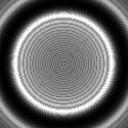
\includegraphics[width=.45\textwidth]{figure/kabs_gray.jpg}} \hspace{10mm} 
    \subfloat[]{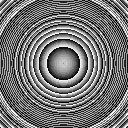
\includegraphics[width=.45\textwidth]{figure/kang_gray.jpg}}
    \bicaption{(a) RSD核幅度图 (b) RSD核相量图。}{(a) The magnitude of an RSD kernel. (b) The phase of an RSD kernel.}
    \label{fig:kernel}
\end{figure}

从式(\ref{eq:kernel})和(\ref{eq:rxy})中可以看出RSD核具有径向对称的特性。如图\ref{fig:kernel},我们也能从RSD核的幅度和相位分布看出这种径向对称的特性。因此,我们可以利用RSD核的这种径向对称性以及傅里叶变换的线性性质,可以显著地减少存储需求以及存储访问次数。图\ref{fig:opt_algo}展示了优化RSD重构算法的基本概念。首先是利用一组RSD核的基函数——半径不同的单位环形脉冲函数——和每个基函数对应的系数,来实时构成傅里叶域的RSD核。同时,如图\ref{fig:opt_algo}(b)通过进一步在径向上采样,基函数可以进一步被一个一维向量重构。最后的结果显示,RSD重构算法执行过程中,总的存储需求以及存储访问次数有了大幅降低。本文将在下面两个小节将详细介绍以上提到上述的两种环形采样和径向采样技术。

\begin{figure}[!tb]
    \centering
    \subfloat[]{\includegraphics[width=.9\textwidth]{figure/opt_algo.pdf}}\\ \vspace{6pt}
    \subfloat[]{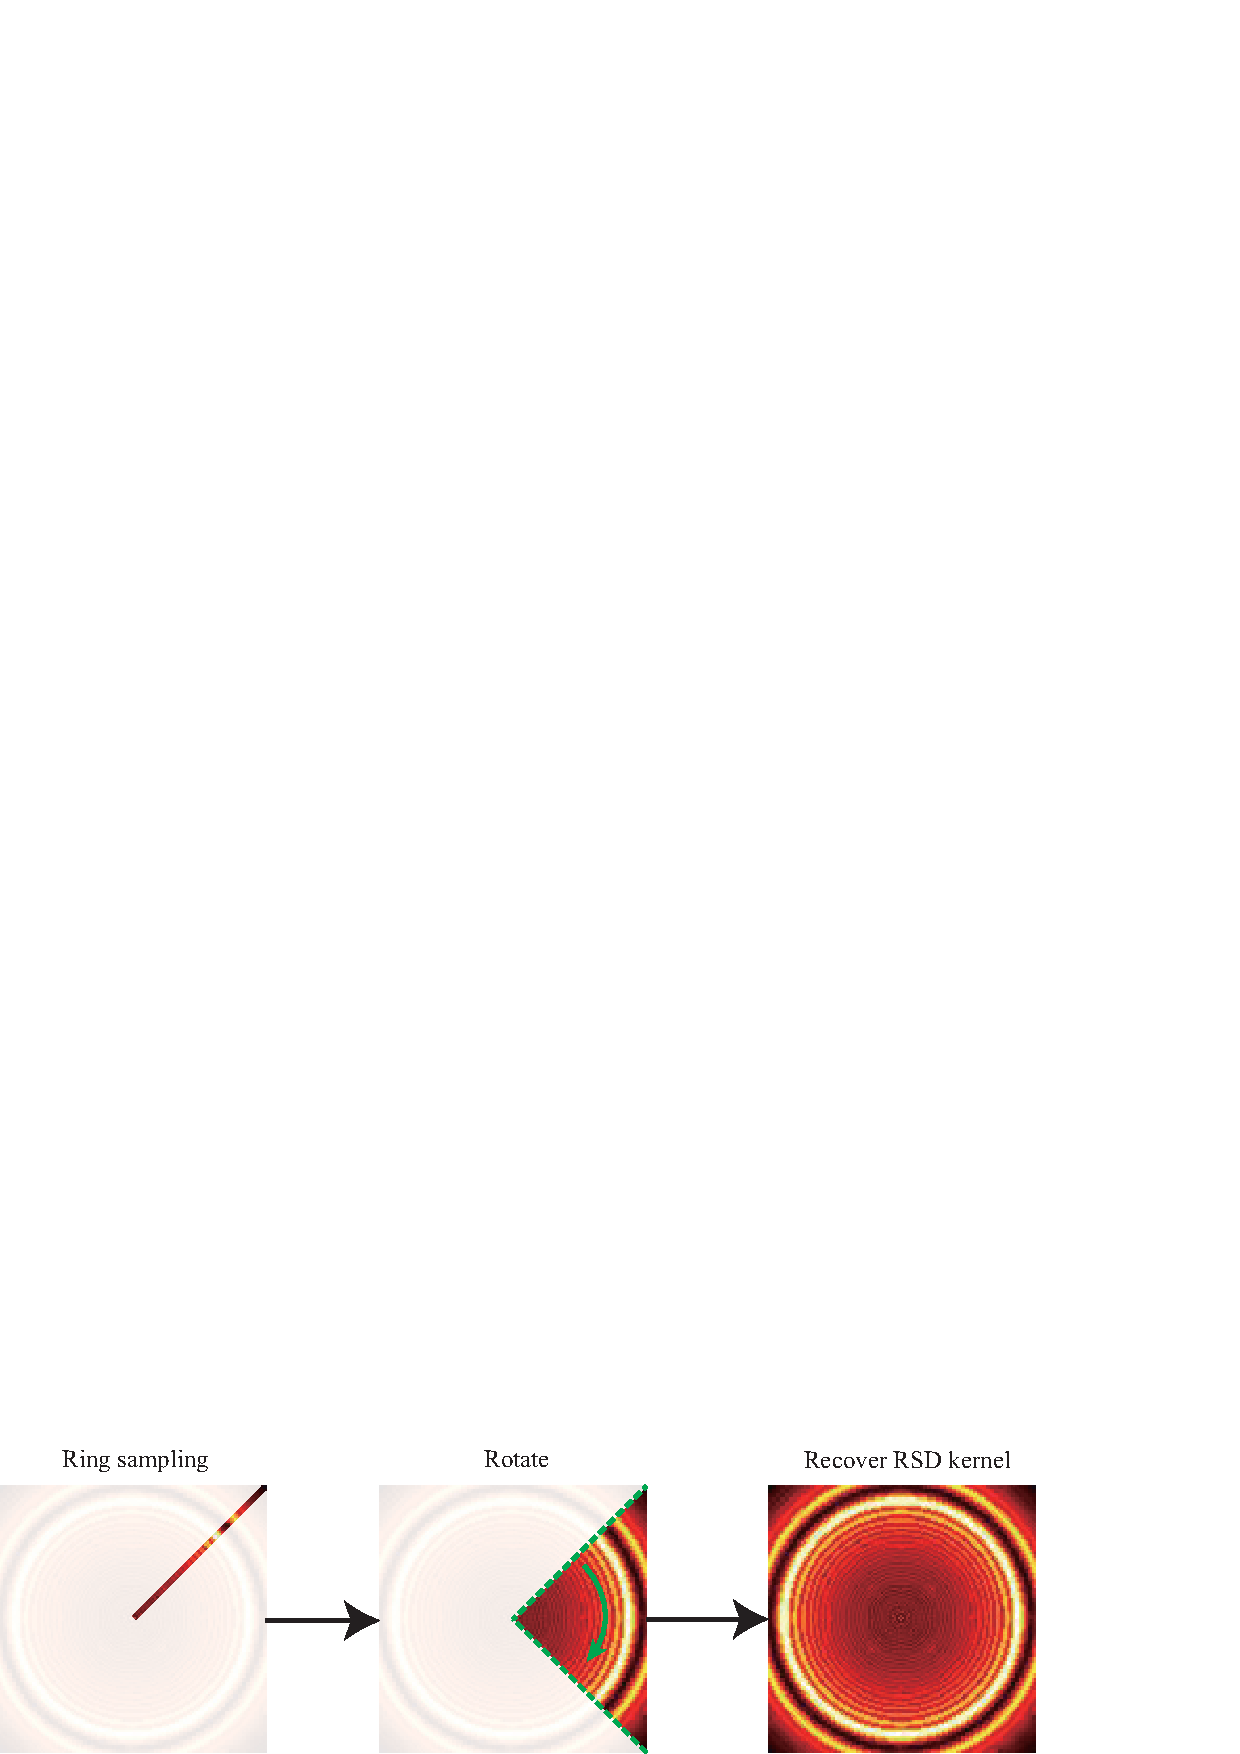
\includegraphics[width=.9\textwidth]{figure/addrmap1.pdf}}
    \bicaption{优化RSD重构算法的基本概念。 (a) 利用单位环形脉冲和对应的系数来重构RSD核。 (b) 利用地址重映射来重构单位环形脉冲。}{Basic concept of the optimized RSD algorithm. (a) Reconstruction of RSD kernels using unit ring impulses and corresponding coefficients. (b) Reconstruction of unit rings using address mapping.}
    \label{fig:opt_algo}
\end{figure}

\subsection{环形脉冲采样技术}

从图\ref{fig:kernel}中可以看出,RSD核是径向对称的,因此其可以如图\ref{fig:opt_algo}(a)被表达为一组有不同半径长度的单位环形脉冲函数的线性组合
\begin{equation}
    G(x, y, \hat{z}, \omega) = \sum_{i=1}^{N_R}\hat{G}(r_i, \hat{z}, \omega)\delta(x, y, r_i)
\end{equation}
其中,单位环形脉冲函数定义为
\begin{equation}
    \delta(x, y, r_i) = \begin{cases}
      1, & \sqrt{x^2+y^2} = r_i\\
      0, & \sqrt{x^2+y^2} \neq r_i
    \end{cases}\label{eq:ring_imp}
\end{equation}
而对应于不同半径的单位环形脉冲函数的线性组合系数为
\begin{equation} \label{eq:ori_coef}
    \hat{G}(r_i, \hat{z}, \omega) = \frac{\exp{\left[-i2\pi\cdot\hat{z}^2/(\eta^2)\cdot\sqrt{r_i^2/\hat{z}^2+1}\right]}}{\sqrt{r_i^2/\hat{z}^2+1}}
\end{equation}
其中,$r_i$是半径长度集合$R$中的第$i$个单位环形脉冲函数的半径。利用傅里叶变换的线性性质,RSD核的傅里叶频域表示为
\begin{equation}
    \mathcal{F}\left[G(x, y, \hat{z}, \omega)\right] = \sum_{i=1}^{N_{ {R}}}\hat{G}(r_i, \hat{z}, \omega)\mathcal{F}\left[\delta(x, y, r_i)\right]
\end{equation}
其中,$\mathcal{F}$表示针对$xy$平面的二维傅里叶变换。根据式(\ref{eq:ring_imp})定义,单位环形脉冲函数可以由$\delta(x,y,r_i)$重新表示为$\delta(r,r_i)$。对于第$i$个单位环形脉冲函数,其傅里叶频域表达为
\begin{equation}
    \begin{split}
        \delta_{\mathcal{F}}(\rho, r_i)&=\int_0^{+\infty}\left(\int_0^{2\pi}e^{-2\pi r\rho \cos (\theta)}d\theta\right)\delta(r, r_i)rdr\\
        &=\int^{2\pi}_0e^{-2\pi r_i\rho \cos \theta}d\theta \cdot r_i = \mathcal{F}\left[ \delta(r,r_i) \right]
    \end{split}
\end{equation}
注意到,只要单位环形脉冲函数的半径$r_i$确定,其对应的频域$\delta_{\mathcal{F}}(\rho,r_i)$的值就是确定的。利用这一点,我们可以预计算好单位环形脉冲函数的频域的值,并存储起来以省略去这一部分的傅里叶变换的计算,从而大大减少算法运行时所需的计算量。由此,RSD核的频域表示可以通过将每个半径的单位环形脉冲函数的频域表示乘以对应半径的线性系数,并将乘积在半径上进行累加来重构。这样的优化可以使得计算RSD核所需的总存储量以及存储访问量大大减少。

\subsection{径向采样技术}

利用径向对称的函数其二维傅里叶变换后的函数同样也是径向对称的性质\cite{baddour2011two},我们可以仅仅利用频域上的单位环形脉冲函数的径向上的值来重构整个函数。这样我们对于单位环形脉冲函数的存储从原来的二维矩阵缩减到了仅仅半径上的一个一维向量,如图\ref{fig:imp_rad}。
\begin{figure}[!tb]
    \centering
    \includegraphics[width=.95\textwidth]{figure/imp30.pdf}
    \bicaption{单位环形脉冲函数在半径上的采样。}{Radius sampling of unit ring impulses.}
    \label{fig:imp_rad}
\end{figure}

如图\ref{fig:opt_algo}(b)所示,若要从一个沿半径采样获得的一维向量中重构出完整的二维单位环形脉冲函数的频域,需要一个二维地址映射从一维向量中找到二维单位环形脉冲函数矩阵中每个元素的值。这一地址映射将矩阵元素的笛卡尔坐标转换为相应的用于描述单位环形脉冲函数的极坐标。理论上,这个地址映射不会有任何影响,但由于这一操作在实际运行时是离散的,我们使用的地址映射函数$M(x,y)$定义如下
\begin{align}
    &s=\sqrt{(x-K/2)^2+(y-K/2)^2}  \\
    &\rho = M(x, y) = round\left( s\cdot \frac{N_{\rho}-1}{\frac{\sqrt{2}}{2}K} \right)+1\label{eq:mapping_func}
\end{align}
其中,$s$是采样点到一个原始的$K\times K$的矩阵中心点的距离,$N_\rho$是半径上采样点的个数。注意到,由于映射函数$M(x,y)$及其操作的对象是离散的,因此利用它来重构RSD核会导致一定程度上的精度损失。图\ref{fig:smp_comp}展示了随着在半径上的采样点个数从10到200的变化,优化后的RSD重构算法所得结果与原始算法结果的相似度变化。这里所用的相似度的测量算法是结构相似度(Structural Similarity,SSIM)。两个图片之间的SSIM值越大表明两者越相似,最大为1时表示两张图片完全相同。从图\ref{fig:smp_comp}中我们可以看到在采样点个数达到了100个以上后,相似度基本持平在0.9左右,而若采样点从100下降到10时,相似度将迅速下降到0.5以下。
\begin{figure}[!tb]
    \centering
    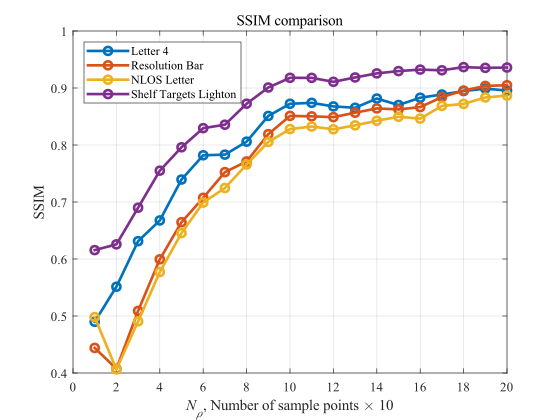
\includegraphics[width=.9\textwidth]{figure/smp_Nrho_comp_ssim.pdf}
    \bicaption{不同的半径采样点个数下,径向采样的重构结果与原始算法的重构结果的相似度对比。}{Similarity measurement between the radius-sampled results and original results, against different numbers of sampling points $N_{\rho}$.}
    \label{fig:smp_comp}
\end{figure}

同样可以看到这一地址映射操作不仅仅可以用在单位环形脉冲函数上,也可以用在RSD核重构上,即地址映射操作在算法处理流程中的次序不会影响到最终RSD核的重构结果。经过径向采样技术对算法的优化,存储单位环形脉冲函数所需的容量从$K\times K$减少到$\frac{\sqrt{2}}{2}K$。

\subsection{优化后的RSD重构算法}\label{sec:opt_algo}

\begin{table}[!t]
    \centering
    \bicaption{原始算法和优化后算法的复杂度比较}{Complexity Comparison between Original and Optimized RSD Algorithms}
    \label{tab:fuzadu_comp}
    % \resizebox{.98\textwidth}{!}{%
        \begin{tabular}{@{}ccc@{}}
            \toprule
            算法               & 计算量 & 存储访问 \\ \midrule
            原始RSD算法 & $O(N_DN_{\Omega}K^2\log K)$          & $O(N_DN_{\Omega}K^2)$             \\
            优化后的RSD算法& $O(N_DN_{\Omega}K^2)$              & $O(N_{\Omega}K^2)$             \\ \bottomrule
        \end{tabular}%
    % }
\end{table}

经过前述两节介绍的优化技巧,优化后的基于RSD的NLOS重构算法由两部分组成:(i)运行前的算法以及(ii)运行时的算法。前者包括单位环形脉冲函数集和相应的线性组合系数的预计算,可以存储在硬件设备上;后者则是利用预计算的数据和实时采集的NLOS成像数据来重构隐藏场景的成像算法,需要在硬件上实时运行。因此这里作为预计算部分的前者不会实际影响到成像系统的整体性能。这两部分的算法伪代码在算法\ref{algo:b_rt}和算法\ref{algo:rt}中有详细说明。

表格\ref{tab:fuzadu_comp}分别展示了原始算法和优化后算法的RSD算法的计算复杂度和存储访问量。如前面章节所讨论的,原始算法中大量的二维傅里叶变换是其瓶颈所在。因此,重构RSD核所需的计算量和存储量在衡量和比较原始算法和优化后的算法之间的复杂度时必须考虑进去。

\begin{algorithm}[!t]
    \caption{运行前算法}
    \label{algo:b_rt}
    \begin{algorithmic}[1] % The number tells where the line numbering should start
        \Require 采样深度$\hat{z}$; 采样频率$\Omega$; 采样半径$r$。
        \Ensure 预计算数据%\\
        \State 求解输入信号的频率响应:
        \For{$q \gets 1, N_{\Omega}$}
            \State $ P_F(x_c, y_c, \omega_q) \gets \sum_t[P(x_c, y_c, t)e^{-i\omega_q t}] $
        \EndFor
        \State 计算单位环形脉冲函数的傅里叶表示:
        \For{$j \gets 1, N_{R}$}
            \For{$k \gets 1, N_{ {\rho}}$}
                \State $$ \delta_{\mathcal{F}}(\rho_k, r_j) \gets \int_0^{2\pi}r_je^{-2\pi r_j \rho_k \cos \theta} d\theta $$
            \EndFor
        \EndFor
        \State 计算线性组合系数:
        \For{$q \gets 1, N_{\Omega}$}
            \For{$p \gets 1, N_D$}
                \For{$k \gets 1, N_R$}
                    \State $$\hat{G}(r_k, \hat{z}_p, \omega_q) \gets \frac{\exp{\left[-i2\pi\cdot\hat{z}_p^2/(\eta^2)\cdot\sqrt{r_k^2/\hat{z}_p^2+1}\right]}}{\sqrt{r_k^2/\hat{z}_p^2+1}}$$
                    \State $$ \hat{G}(r_k, \hat{z}_p, \omega_q) \gets \hat{G}(r_k, \hat{z}_p, \omega_q) \cdot \exp\left[i\frac{\omega_q}{c}(\hat{z}_p+B_l)\right] $$
                \EndFor
            \EndFor
        \EndFor
        % \State Generate address mapping matrix 
        % $$
        %     M_{xy} \gets round\left( \frac{\sqrt{(x-K/2)^2+(y-K/2)^2}}{K/2*\sqrt{2}/(N_{ {r}}-1)} \right)+1
        % $$
    \end{algorithmic}
\end{algorithm}

\begin{algorithm*}[!t]
    \caption{Algorithm at runtime}
    \label{algo:rt}
    \begin{algorithmic}[1]
        \Require 瞬态图像$P_F$; 环形脉冲$\delta_{\mathcal{F}}$; 组合系数$\hat{G}$
        \Ensure 重构结果$I$
        \Procedure{Reconstruction}{$P_F, \delta_{\mathcal{F}}, \hat{G}$}
        \For{$i \gets 1, N_{ {D}}$}\Comment{循环1:采样深度上迭代}
            \For{$j \gets 1, N_{ {\Omega}}$}\Comment{循环2: 采样频率上迭代}
                \State $\mathcal{P}_F(x, y, \omega_j) \gets FFT2(P_F(x, y, \omega_j))$
                \For{$k \gets 1, N_{ {R}}$}\Comment{不同半径上迭代}
                    \For{$l \gets 1, N_{\rho}$}\Comment{所有径向采样点上迭代}
                        \State $G(\rho_l, \hat{z}_i, \omega_j) \gets G(\rho_l, \hat{z}_i, \omega_j) + \hat{G}(r_k, \hat{z}_i, \omega_j)\cdot \delta_{\mathcal{F}}(r, r_k) $
                    \EndFor
                \EndFor
                \For{$x \gets 1, K$} \Comment{在所有坐标上迭代}
                    \For{$y \gets 1, K$}
                        \State $G^{\prime}(x, y, \hat{z}_i, \omega_j) \gets G(M(x, y), \hat{z}_i, \omega_j)$ \Comment{地址映射}
                        \State $ S_F(x, y, \hat{z}_i, \omega_j) \gets \mathcal{P}_F(x, y, \omega_j) \cdot G^{\prime}(x, y, \hat{z}_i, \omega_j) $ 
                    \EndFor
                \EndFor
                \State $I_F(x, y, \hat{z}_i) \gets I_F(x, y, \hat{z}_i) + S_F(x, y, \hat{z}_i, \omega_j)$ \Comment{对所有采样频率累加}
            \EndFor
            \State $I(x, y, \hat{z}_i) \gets IFFT2 \left[ I_F(x, y, \hat{z}_i) \right]$ \EndFor 
        % Do 2D inverse Fourier transformation
        \EndProcedure
    \end{algorithmic}
\end{algorithm*}

\chapter{RSD重构算法加速电路设计}
这一章将对实时NLOS重构算法\ref{algo:rt}进行深入分析,并讨论其引入的一些设计上的挑战。

\section{重构算法的分析} 

\subsection{任务流程分析}
运行时NLOS重构算法的流程图如图\ref{fig:tsk_flow}所示。整个算法流程中存在四个计算密集和存储访问密集的任务:
\begin{enumerate}
  \item 由单位环形脉冲函数和线性组合系数重构RSD核。
  \item 对输入瞬态图像的二维傅里叶变换。
  \item RSD核与瞬态图像的频域做的乘累加操作。
  \item 对累加结果的二维反傅里叶变换。
\end{enumerate}
\begin{figure}[!tb]
    \centering
    \includegraphics[width=.99\textwidth]{figure/taskflow.pdf}
    \bicaption{运行时重构算法的流程图}{Flowchart of the runtime reconstruction algorithm.}
    \label{fig:tsk_flow}
\end{figure}

整个重构过程可以被分割成$N_D\times N_\Omega$个执行周期。其中每个执行周期用深度计数器和频率计数器的值以$(d,f)$形式标记,因此整个重构过程由执行周期$(0,0)$开始,一直迭代到最后一个执行周期$(N_D-1,N_\Omega-1)$。在以上四个任务中,任务1到任务3在每个执行周期均会被执行,而任务4则只在频率计数器$f$计数至$N_\Omega$时执行。我们可以看到任务1和任务2时相互独立的,因此它们可以被并行执行。而任务3——乘累加任务——则是对任务1和任务2的结果有所依赖。一旦频率计数器计满至$N_\Omega$,任务3乘累加的结果被输入给任务4,以重构相应于深度计数器值的深度的隐藏场景。输入的瞬态图像可以表示为一个多通道的图像,一个$K\times K\times N_\Omega$的张量,单位环形脉冲函数总体表示为一个$N_R\times N_\rho$的矩阵,其线性组合系数则可以表示为一个$N_D\times N_\Omega\times N_R$张量。

对每一个执行周期,二维傅里叶变换处理器需要读取$K\times K$个像素,并输出其傅里叶变换后的结果。假设瞬态图像的输入通道的传输速率为每个时钟周期传送一个像素,那么一共需要$K\times K\times N_D\times N_\Omega$个时钟周期来读取整个瞬态图像。对于一个典型的NLOS成像系统配置\cite{Liu2020},其中各个参数配置为$K=128, N_D=51, N_\Omega=69$,读取瞬态图像一共需要耗费57655296个时钟周期。我们可以自然地想到一个解决这一问题的想法,即仅仅对所有采样频率点上的瞬态图像做一次二维傅里叶变换,并将其结果存储在本地,随后的执行周期复用这一结果即可。这样一来,好处是可以将读取时间降低至$K\times K\times N_\Omega$个时钟周期,而坏处则是需要更大的片上存储单元来缓存中间结果。

\subsection{线性组合系数分解}

在章节\ref{sec:opt_algo}分析优化后的基于RSD的NLOS重构算法时,我们将线性组合系数的计算放在运行前算法部分,作为与计算的结果存储在本地供运行时算法使用。好处是可以降低运行时的计算负载,但坏处则是引入很大的存储需求。这里,为了进一步降低片上存储单元的使用量,微调了两部分算法的切分,将一部分线性组合系数的计算转移至运行时。注意到,由于傅里叶变换的线性性质,时移因子$T_l$可以被合并至线性组合系数$\hat{G}$里。因此,对应于单位环形脉冲函数的线性组合系数\ref{eq:ori_coef}可以被重新定义为
\begin{align} \label{eq:coef}
    \hat{G}(r, \hat{z}, \omega) & = \frac{\exp{\left[-i2\pi\cdot\frac{\delta \omega\hat{z}}{\mathbf{c}}\cdot\sqrt{r^2/\hat{z}^2+1}\right]}}{\sqrt{r^2/\hat{z}^2+1}}\\
    \tilde{G}(r, \hat{z}, \omega) & = \hat{G}(r, \hat{z}, \omega) \cdot T_l 
\end{align}
这里,我们引入三个独立的中间变量来进一步分解上述定义的线性组合系数,
\begin{equation}
    W(r, \hat{z}) = \sqrt{\frac{r^2}{\hat{z}^2}+1}
\end{equation}
\begin{equation}
    D(\omega, \hat{z}) = \frac{\delta \omega \hat{z}}{\mathbf{c}}
\end{equation}
\begin{equation}
    T(\omega, \hat{z}) = T_l= \exp \left[ i\frac{\omega}{\mathbf{c}}(\hat{z}+B_l) \right]
\end{equation}
这三个中间变量可以利用选取好的采样深度$\hat{z}$,采样频率$\omega$,以及不同的环形半径$r$来预先计算,并存储为三个可以被深度计数器$d$和频率计数器$f$索引的矩阵。在本文中,我们将这三个变量$W,D,T$分别命名为\textit{wave, distance}和\textit{timeshift}. 而上述重新定义的线性组合系数可以被这三个中间变量重新组合
\begin{equation}
    \tilde{G}(r, \omega, \hat{z}) = \frac{\exp(-i2\pi W(r, \hat{z}) \cdot D(\omega, \hat{z}))}{W(r, \hat{z})} \cdot T(\omega, \hat{z})
\end{equation}

在运行时,加速器将会在每个执行周期读取$D$和$T$的一个元素,并在频率计数器$f=0$的执行周期,$(0,0),(1,0)$……$(N_D-1,0)$内读取$W$的一列元素。对系数的重新组合过程可以由一些基本的运算部件来承担,如两个乘法器、一个除法器以及一个处理特殊函数
\begin{equation}
    f(t) = e^{-i2\pi t}
\end{equation}
的计算单元。这里的系数分解方法仅仅是为了在设计复杂度、片上存储单元面积大小以及存储访问次数之间取得均衡所做的取舍,同时在不对系统造成性能上的负面影响的前提下尽量提升功耗和面积效率的一种手段。

\section{设计空间探索}

本章节将会引入一些主要的NLOS成像加速器设计参数来定量化的描述设计空间,以探索数据流优化的最佳参数配置。

\chapter{加速电路的微架构设计}
% \shtthesis{} 实际使用 \CTeX 宏包提供的 \textsf{ctexbook} 文档类排版,除上述选项外的类参数会传递给 \textsf{ctexbook}。其中需要注意的选项为 \verb|fontset|,即设定论文所用的字体集。\CTeX 宏包自身能够根据编译平台选择合适的字体集,也可以手动设置相应的 fontset,例如在 Windows 平台下设置 \verb|fontset=windows|,在 macOS 平台下设置 \verb|fontset=mac|:
% \begin{latex}
% \documentclass[fontset=windows]{shtthesis}
% \end{latex}
% 不同字体集所用字体见表~\ref{tab::fonts}。在 Linux/UNIX 环境下对于宋体和黑体,会首先检测思源宋体/黑体(Source Han 字体或 Noto CJK 字体)是否安装,若未检测到则回退至 Fandol 宋体/黑体;对于楷体和仿宋,则会依次检测方正楷体/仿宋-GBK 是否安装,若未检测到则退回至 Fandol 楷体/仿宋。

% \begin{table}[htb]
%   \centering
%   \caption{不同字符集下 \shtthesis{} 所用字体}
%   \label{tab::fonts}
%   \begin{subtable}{\columnwidth}
%     \centering
%     \caption{\shtthesis{} 所用中文字体}
%     \label{tab::chs_fonts}
%     \begin{tabular}{*{3}{c}}
%       \toprule
%       Windows & macOS & Linux/UNIX \\
%       \midrule
%       \songti   中易宋体 & \songti   华文宋体简体 & \songti   思源宋体 $\to$ Fandol 宋体 \\
%       \heiti    中易黑体 & \heiti    华文黑体简体 & \heiti    思源黑体 $\to$ Fandol 黑体 \\
%       \kaishu   中易楷体 & \kaishu   华文楷体简体 & \kaishu   方正楷体-GBK $\to$ Fandol 楷体 \\
%       \fangsong 中易仿宋 & \fangsong 华文仿宋简体 & \fangsong 方正仿宋-GBK $\to$ Fandol 仿宋 \\
%       \bottomrule
%     \end{tabular}
%   \end{subtable}
%   \newline
%   \vspace{12pt}
%   \newline
%   \begin{subtable}{\columnwidth}
%     \centering
%     \caption{\shtthesis{} 所用英文字体(全平台一致)}
%     \label{tab::eng_fonts}
%     \begin{tabular}{*{3}{c}}
%       \toprule
%       \textrm{Serif} & \textsf{Sans Serif} & \texttt{Typewriter} \\
%       \midrule
%       \textrm{\TeX{} Gyre Termes} & \textsf{\TeX{} Gyre Heros} & \texttt{\TeX{} Gyre Cursor} \\
%       \bottomrule
%     \end{tabular}
%   \end{subtable}
% \end{table}

% 需要注意 Fandol 系列字体虽然为 \TeX{} Live 自带,但其字符覆盖有限,对于生僻字可能出现缺字情况。可以通过查看附录~\ref{sec::chs_rare} 确认当前编译环境所用的字体库是否有缺字风险。思源宋体\footnote{\url{https://source.typekit.com/source-han-serif/cn/}}、思源黑体\footnote{\url{https://github.com/adobe-fonts/source-han-sans}}、方正楷体-GBK\footnote{\url{https://www.foundertype.com/index.php/FontInfo/index/id/137}}和方正仿宋-GBK\footnote{\url{https://www.foundertype.com/index.php/FontInfo/index/id/128}} 均为免费字体且完整覆盖简繁扩展 (GBK) 字符集,非常推荐 Linux/UNIX 用户安装使用。

\section{微架构概述} \label{sec::setup_info}
% 知晓学位类型后,\shtthesis{} 还需其他必要信息才能进行进一步排版:根据《规范》,博士学位论文和硕士学位论文需要在中英文封面中,依次列出论文密级、论文标题、作者姓名、导师信息、学位类别、一级学科、学校/学院名称及论文完成时间;根据\citet{bachelor2019},本科生学位论文需要在中英文封面中依次列出论文题目、学生姓名、学号、入学年份、学院、专业、指导教师及论文完成时间。以上信息均可通过 \verb|\shtsetup| 命令,在论文导言区(即 \verb|\documentclass| 之后、\verb|\begin{document}| 之前)以 key=value 方式统一设定。用户可以一次性调用 \verb|\shtsetup| 设定所有信息,也可分多次设定。

% 研究生论文信息设定样例为:
% \begin{latex}
% \shtsetup{
%   degree-name = {工学硕士},
%   degree-name* = {Master~of~Science~in~Engineering},
%   secret-level = {白给},
%   title = {\ShtThesis{}~v\version{}~使用说明},
%   title* = {A~User's~Guide\\to\\\ShtThesis{}~v\version{}},
%   keywords = {非视域成像,瑞利索墨菲散射,硬件加速,现场可编程逻辑门阵列},
%   keywords* = {Non-light-of-sight imaging (NLOS), Rayleigh-Sommerfeld Diffraction (RSD), Hardware accelerator, Field programmable gate array (FPGA)},
%   author = {李润东},
%   author* = {Li~Rundong},
%   institution = {上海科技大学信息科学与技术学院},
%   institution* = {School~of~Information~Science~and~Technology\\%
%                   ShanghaiTech~University},
%   supervisor = {范睿~副教授},
%   supervisor* = {Professor~Fan~Rui},
%   supervisor-institution = {上海科技大学信息科学与技术学院},
%   discipline-level-1 = {计算机科学与技术},
%   discipline-level-1* = {Computer~Science~and~Technology},
%   date = {2020~年~6~月},
%   date* = {June,~2020},
%   bib-resource = {reference.bib},
% }
% \end{latex}

% 本科生论文信息设定样例为:
% \begin{latex}
% \shtsetup{
%   title = {\ShtThesis{}~v\version{}\\使用说明},
%   title* = {A~User's~Guide~to\\\ShtThesis{}~v\version{}},
%   keywords = {上海科技大学,学位论文,\LaTeX{}},
%   keywords* = {ShanghaiTech~University, Thesis, \LaTeX{}},
%   date = {2020~年~06~月},
%   date* = {06~/~2020},
%   author = {李润东},
%   author* = {Rundong~Li},
%   author-id = {36273800},
%   entrance-year = {2017},
%   institution = {信息科学与技术学院},
%   institution* = {School~of~Information~Science~and~Technology},
%   supervisor = {范睿},
%   supervisor* = {Rui~Fan},
%   discipline = {计算机科学与技术},
%   discipline* = {Computer~Science~and~Technology},
%   bib-resource = {reference.bib},
% }
% \end{latex}

% 在 \verb|\shtsetup| 的 key=value 设定机制中,表示中文信息条目的 key 为 \verb|-| 连接的小写单词(例如研究生学位中文名称 \verb|degree-name|),由 \verb|*| 结尾的 key 一般表示对应的英文条目(例如研究生学位英文名称 \verb|degree-name*|);value 可以在前后添加大括号,也可以不添加。特别需要注意 \verb|\shtsetup| 命令内\emph{不能有空行}。

\section{RSD卷积核生成器}
% 研究生学位论文需要额外设定的学位信息包括:学位名称(degree-name)和英文学位名称(degree-name*),具体见表~\ref{tab::degree_info}。学位类型会影响 \shtthesis{} 的中英文封面内容。
% \begin{table}[htb]
% \centering
% \caption{通过\texttt{shtsetup}设定的学位信息} \label{tab::degree_info}
% \begin{tabular}{llp{0.5\columnwidth}}
%   \toprule
%   key & value 样例 & 说明 \\
%   \midrule
%   degree-name & 学术型博士 & 中文学位名称,《规范》中学术型学位中文名称包括:\emph{学术型博士}、\emph{理学硕士}、\emph{工学硕士} \\
%   degree-name* & Doctor~of~Philosophy & 英文学位名称,《规范》中上述学位对应的英文名称为:\emph{Doctor~of~Philosophy}、\emph{Master~of~Natural~Science}、\emph{Master~of~Science~in~Engineering} \\
%   \bottomrule
% \end{tabular}
% \end{table}

\section{二维快速傅里叶变换模块}
% 设定论文中英文标题和涉密等级。中文标题(title)和英文标题(title*)中可以包含换行符。研究生学位论文的涉密等级(secret-level)会以“密级:\uline{XXX}”显示在中文封面右上角,未设定涉密等级则不显示相关信息。

\section{乘累加阵列}
% 需要设定的作者信息包括:作者中英文姓名(author 和 author*)和学校/学院中英文名称(institution 和 institution*),研究生需要设定一级学科中英文名称(discipline-level-1 和 discipline-level-1*),本科生需要设定攻读专业中英文名称(discipline 和 discipline*)。

% 特别注意研究生和本科生的英文名格式要求不一致:研究生要求以姓氏拼音在前、名字拼音在后、中间以半角空格分隔的格式书写英文姓名:
% \begin{latex}
% \shtsetup{
%   % 研究生中英文姓名格式要求
%   author = 李润东,
%   author* = {Li~Rundong}, % 正确写法
%   % author* = {Rundong~Li}, % 错误写法
% }
% \end{latex}
% 而本科生要求以名字拼音在前、姓氏拼音在后、中间以半角空格分隔的格式书写英文姓名:
% \begin{latex}
% \shtsetup{
%   % 本科生中英文姓名格式要求
%   author = 李润东,
%   author* = {Rundong~Li}, % 正确写法
%   % author* = {Li~Rundong}, % 错误写法
% }
% \end{latex}

% 研究生需要设定完整的学校、学院名称,中文名称(institution)不可带换行符,英文名称(institution*)应在学院、学校名称间加入换行符,否则封面排版会出现错误:
% \begin{latex}
% \shtsetup{
%   institution = 上海科技大学信息科学与技术学院,
%   institution* = {School~of~Information~Science~and~Technology\\%
%                   ShanghaiTech~University},
% }
% \end{latex}
% 本科生则不必包含学校名称,直接设定学院名称即可,注意中英文名称中均不能包含换行符:
% \begin{latex}
% \shtsetup{
%   institution = 信息科学与技术学院,
%   institution* = {School~of~Information~Science~and~Technology},
% }
% \end{latex}

\section{后处理模块}
% 需要设定的导师信息包括:导师中英文姓名(supervisor 和 supervisor*)和导师单位中文名称(supervisor-institution)。注意在中文封面中,导师姓名和单位分两行显示在“指导教师”条目下。根据《规范》,导师中文姓名(supervisor)应包含导师职称,如教授、副教授、助理教授、研究员、副研究员,以一个半角空格跟随在姓名之后;导师英文姓名(supervisor*)则统一以“Professor”开头,与英文姓名以一个半角空格隔开。导师单位中文名称(supervisor-institution)不可包含换行符。
% \begin{latex}
% \shtsetup{
%   supervisor = {范睿~副教授},
%   supervisor* = {Professor~Fan~Rui},
%   supervisor-institution = {上海科技大学信息科学与技术学院},
% }
% \end{latex}

\chapter{硬件实现结果}
% 通过 date 和 date* 分别设置中英文成文日期,日期内容应按照申请学位的时间节点填写,具体请参考当年《规范》。研究生成文日期格式为:
% \begin{latex}
% \shtsetup{
%   date = {2020~年~6~月},
%   date* = {June,~2020},
% }
% \end{latex}
% 本科生成文日期格式为:
% \begin{latex}
% \shtsetup{
%   date = {2020~年~06~月},
%   date* = {06~/~2020},
% }
% \end{latex}

\section{优化后算法的重构结果比较}
% 《规范》规定论文前言部分应包含论文原创性声明和授权使用声明、中英文摘要、目录,研究生论文还需包含图形、表格列表。若有需要,可加入符号列表。\shtthesis{} 会自动生成目录和图表列表,在不设置 \verb|anonymous| 选项时会自动生成声明页。\shtthesis{} 提供了摘要和符号列表环境,以便于用户生成中英文摘要和符号列表。

\section{FPGA实现结果}
% 论文中英文摘要在正文部分 \verb|\frontmatter| 之后、\verb|\makeindices| 之前,分别在 abstract 和 abstract* 环境中输入。摘要环境对内容没有限制:
% \begin{latex}
% \begin{abstract}
%   中文摘要内容...
% \end{abstract}

% \begin{abstract*}
%   English abstract content...
% \end{abstract*}
% \end{latex}

% 需要注意,本科生论文要求在中英文摘要中包含论文标题。默认情况下,\shtthesis 的 abstract 和 abstract* 环境会按照 \verb|\shtsetup| 中指定的标题及其中的换行符进行排版。如果希望在摘要中显示的标题不换行,则可以向摘要环境传入 \verb|flattitle| 选项,排版时会将 title 和 title* 中的换行符替换为空格:
% \begin{latex}
% \begin{abstract}[flattitle]
%   % 摘要标题排版时不换行
%   中文摘要内容...
% \end{abstract}
% \end{latex}

% 论文中英文关键词在 \verb|\shtsetup| 命令中分别以 keywords 和 keywords* 设定。注意 \shtthesis{} v\version{} 中尚未实现分词处理,此处输入的 value 将不经任何预处理,直接插入至正文中排版。因此,中文关键词(keywords)之间应该以中文逗号“,”隔开且不包含空格;英文关键词(keywords*)之间应该以半角逗号“,”隔开,并在每一半角逗号后跟随一个半角空格。
% \begin{latex}
% \shtsetup{
%   keywords = {上海科技大学,学位论文,\LaTeX{}},
%   keywords* = {ShanghaiTech~University, Thesis, \LaTeX{}},
% }
% \end{latex}

\chapter{总结与展望}
% \shtthesis{} 重载了 \verb|\makeindices| 命令,可一次生成目录、图形列表和表格列表。默认目录中正文标题列出至第 3 级(即 subsection),若包含附录则目录中只列出“附录”一项(附录各级标题仍会生成 PDF 书签),图形、表格列表中列出图表标题的全部内容。对于特别长的图形、表格标题,可以在 \verb|\caption| 命令中指定短标题,从而使列表条目更为简明:
% \begin{latex}
% \begin{figure}
%   \caption[出现在图形列表内的短标题]{出现在正文中的长标题}
%   % ...
% \end{figure}
% \end{latex}

% \shtthesis{} 提供了 nomenclatures 环境用于在研究生论文中生成符号列表,其使用方法为:
% \begin{latex}
% \begin{nomenclatures}[<标题>]
%   \head[<单位表头>]{<符号表头>}{<描述表头>}
%   \item[<单位>]{<符号>}{<描述>}
%   % ...
% \end{nomenclatures}
% \end{latex}
% 每次 nomenclatures 调用会分别生成一组符号列表,每一 \verb|\item| 会生成一行符号描述。若 \verb|<标题>| 不为空则会为当前组生成一个不编号的 section 级的标题。\verb|\head| 为可选指令,会为当前组生成一个“表头”,但必须在 \verb|\item| 之前列出。\verb|\item| 接受一个可选参数 \verb|<单位>| 作为符号的单位,若其不为空则在当前行右对齐出现。nomenclatures 的使用样例可以参考 \jobname.tex 中“符号列表”部分。注意在 \shtthesis{} v\version{} 中各 \verb|\item| 的 \verb|<描述>| 在折行后会出现排版错误,故暂时不支持较长的符号描述。

% \chapter{致谢}
% \shtthesis{} 正文部分的书写与一般 \LaTeX 项目无异。\shtthesis{} 为研究生论文修改公式编号格式以符合《规范》要求,并提供编号定理、证明等常用数学环境。文献引用遵循 GB/T 7714-2015 《信息与文献 参考文献著录规则》标准,其中本科论文使用顺序编码制,研究生论文使用“著者-出版年”制。

% \subsection{编号公式}
% 在排版研究生论文时,\shtthesis{} 通过 \textsf{mathtools} 宏包在公式编号前添加 $\ldots$ 以符合《规范》对公式编号的格式要求,如:
% \begin{align}
% P(A|B) &= \frac{P(A)P(B|A)}{P(B)} \label{eq::bayesian}
% \end{align}
% 同时重载了 \verb|\eqref|,使得公式编号格式修改后,其引用格式仍与 \textsf{amsmath} 无异:贝叶斯定理~\eqref{eq::bayesian}。排版本科生论文时不修改公式编号格式。

% \shtthesis{} 使用 \textsf{unicode-math} 宏包进行公式排版,因此在数学环境内既可以用标准 \LaTeX{} 宏,也可以直接输入 Unicode 符号。例如 $\oiint$ 符号可以通过 \verb|\oiint| 宏录入,也可以通过 Unicode 符号 $∯$ (对应 \verb|U+0222F| 码点) 录入。以下测试公式来自 \citet{clerkma2013unicode},其中所有字符均直接使用对应 Unicode 符号录入。
% \begin{align}
% & ⊢ ∀x[(Fx ∨ Gx) → \mathord{∼}Hx] \\
% & ⊨ ¬∃y∀x[x∈y ↔ x∉x]  \\
% & ⊭ x ∩ (y ∪ z) ≠ (x ∩ y) ∪ (x ∩ z) \\
% & ⊢ ⟦α⟧ = ℵ₀ → α ≇ ℘(α) \\
% & ⌜ψ[(℩x)φx]⌝ ≝ ⌜(∃x)[φx ∧ (∀z)(φz ⊃ x=z) ∧ ψx]⌝ \\
% & ⊢ (P ⥽ Q) ⥽ (□P ⥽ ◇Q)
% \end{align}

% \subsection{数学环境}
% \shtthesis 通过 \textsf{amsthm} 宏包定义了常用的数学环境和证明环境,如表~\ref{tab::math_envs} 所列。其中,英文表示 tex 文档内调用的环境名称,中文表示排版后论文中显示的环境名称。

% \begin{table}[htb]
% \centering
% \caption{\shtthesis 提供的数学环境}
% \label{tab::math_envs}
% \begin{tabular}{*{5}{c}}
%   \toprule
%   theorem & lemma & corollary & proposition & conjecture \\
%   定理    & 引理  & 推论       & 命题        & 猜想       \\
%   \midrule
%   definition & axiom & example & problem & exercise \\
%   定义       & 公理  & 例       & 问题    & 练习     \\
%   \midrule
%   remark & & & & \\
%   注 & & & & \\
%   \bottomrule
% \end{tabular}
% \end{table}

% \begin{theorem}[Unicode-CJK 覆盖定理] \label{thm::CJK}
%   Unicode 能够编码绝大多数东亚文字和符号。
% \end{theorem}

% \begin{corollary}
%   Unicode 能够编码我国《汉字内码扩展规范》中的所有字符。
% \end{corollary}

% \begin{corollary}
%   Unicode 也能够编码韩文和日文字符。
% \end{corollary}

% \begin{example}
%   “你好”在 Unicode 中的编码 (codepoints) 为 \verb|U+4F60| 和 \verb|U+597D|。
% \end{example}

% \begin{example}
%   「こんにちは」在 Unicode 中的编码 (codepoints) 为 \verb|U+3053|、 \verb|U+3093|、 \verb|U+306B|、 \verb|U+3061| 和 \verb|U+306F|。
% \end{example}

% \begin{proof}
%   留作练习。使用前请留意注~\ref{rmk::qed} 的提示。
% \end{proof}

% \begin{remark}
%   对定理~\ref{thm::CJK} 感兴趣的读者可以查阅 Unicode 规范(\url{https://unicode.org/})。
% \end{remark}

% \begin{remark} \label{rmk::qed}
%   使用 \hologo{LuaLaTeX} 引擎编译时,证明环境的 QED 符号 $\QED$ 可能会排版出错。
% \end{remark}

% \subsection{文献引用} \label{sec::citation}
% \shtthesis{} 通过 \textsf{biblatex} 宏包及 \textsf{biblatex-gb7714-2015} 格式支持符合 GB/T 7714-2015 标准的文献引用。本科生论文使用顺序编码制,研究生论文使用“著者-出版年”制。

% \paragraph{顺序编码制}
% 使用一般引用 \verb|\cite| 的编码显示为上标,例如~\cite{stamerjohanns2009mathml, yuan2012lana}。也可以使用行内引用 \verb|\inlinecite| 将引用编码排版至正文,例如 \inlinecite{Bohan1928}。参考文献列表按照各条目在正文中被引用顺序排列。

% \paragraph{“著者-出版年”制}
% 使用 \verb|\citet| 进行文本形式的引用 \citet{Bohan1928},使用 \verb|\citep| 进行括号形式的引用 \citep{yuan2012lana},使用 \verb|\citeauthor| 进行作者引用 \citeauthor{niu2013zonghe},以及使用 \verb|\citeyear| 进行年份引用 \citeyear{walls2013drought}。参考文献列表各条目按照语言分组后,按照字母序排列。

% \shtthesis{} 通过 \verb|\shtsetup| 的 bib-resource 选项指定参考文献数据库,例如载入 reference.bib 文件:
% \begin{latex}
% \shtsetup{
%   bib-resource = {reference.bib},
% }
% % ...
% \begin{document}
%   % ...
%   \makebiblio
% \end{latex}

% 需要注意若文献条目的作者姓名非英文,则需额外增加 key 字段指定作者英文姓名,并在姓氏拼英后加注音调,以确保文献条目在文末的参考文献中正确排列。例如 \citet{bravo1990comparative} 无需额外处理,而 \citet{chen1980zhongguo} 对应的 bib 条目需修改为
% \begin{latex}
% @incollection{chen1980zhongguo,
%   author    = {陈晋镳 and 张惠民 and 朱士兴 and 赵震 and 王振刚},
%   key       = {Chen2 Jing Ao Zhang1 Hui Ming Zhu1 Shi Xing Zhao4 Zhen Wang2 Zhen Gang},
%   title     = {蓟县震旦亚界研究},
%   editor    = {中国地质科学院天津地质矿产研究所},
%   booktitle = {中国震旦亚界},
%   address   = {天津},
%   publisher = {天津科学技术出版社},
%   year      = {1980},
%   pages     = {56--114},
% }
% \end{latex}

% \subsection{列表环境}
% \shtthesis{} 微调了编号列表(enumerate)和非编号列表(itemize)环境,以适应中文排版惯例。编号列表默认使用数字编号:
% \begin{enumerate}
%   \item 起来,饥寒交迫的奴隶!
%   \item 起来,全世界受苦的人!
%   \item 满腔的热血已经沸腾,
%   \item 要为真理而斗争!
% \end{enumerate}
% 也可以在 \verb|\begin{enumerate}| 之后,以短标签(short label)形式指定编号格式。例如,使用小写字母+半角括号作为编号:
% \begin{enumerate}[a)]
%   \item 旧世界打个落花流水,
%   \item 奴隶们起来,起来!
%   \item 不要说我们一无所有,
%   \item 我们要做天下的主人!
% \end{enumerate}
% 还可以通过 \verb|resume*| 参数,“继续”被中断的列表编号:
% \begin{enumerate}[a), resume*]
%   \item 这是最后的斗争,
%   \item 团结起来到明天,
%   \item 英特纳雄耐尔
%   \item 就一定要实现!
% \end{enumerate}

% 关键字(description)环境在每一条目关键字后增加了加粗全角冒号“\textbf{:}”以适应中文排版惯例。例如:《中华人民共和国劳动法》
% \begin{description}
%   \item[第一章第三条] 劳动者享有平等就业和选择职业的权利、取得劳动报酬的权利、休息休假的权利、获得劳动安全卫生保护的权利、接受职业技能培训的权利、享受社会保险和福利的权利、提请劳动争议处理的权利以及法律规定的其他劳动权利。
%   \item[第四章第三十六条] 国家实行劳动者每日工作时间不超过八小时、平均每周工作时间不超过四十四小时的工时制度。
%   \item[第四章第四十一条] 用人单位由于生产经营需要,经与工会和劳动者协商后可以延长工作时间,一般每日不得超过一小时;因特殊原因需要延长工作时间的,在保障劳动者身体健康的条件下延长工作时间每日不得超过三小时,但是每月不得超过三十六小时。
%   \item[第四章第四十三条] 用人单位不得违反本法规定延长劳动者的工作时间。   
% \end{description}

% \subsection{双语图表标题}
% 《规范》要求正文中所有图形、表格标题使用中英双语。此需求可以通过 \textsf{bicaption} 宏包实现,如图~\ref{img::sht_logo} 所示。
% \begin{figure}[htb]
%   \centering
%   \IfFileExists{shanghaitech-emblem.pdf}{%
%     \includegraphics[width=0.5\columnwidth]{shanghaitech-emblem.pdf}%
%   }{%
%     \fbox{%
%       \begin{minipage}[b][2.5cm][c]{0.75\columnwidth}%
%         \centering\zihao{-5}\bfseries\sffamily\color{ShtRed}%
%         校徽文件 \texttt{shanghaitech-emblem.pdf} 缺失%
%       \end{minipage}%
%     }%
%   }%
%   \bicaption{上海科技大学校徽}{The emblem of ShanghaiTech University}
%   \label{img::sht_logo}
% \end{figure}

% 由于在排版较长的、自包含的图表标题时,使用双语图表标题会导致可读性下降,\shtthesis{} 默认不载入 \textsf{bicaption} 宏包。( \shtthesis{} 作者在 2020 年学位申请时并未使用双语标题。)若确实需要双语标题,可在导言区内手动载入 \textsf{bicaption}。注意需要设定 \verb|list=off| 以确保英文标题不出现在图表列表中:
% \begin{latex}
% \usepackage[list=off]{bicaption}
% \captionsetup[figure][bi-second]{name=Figure}
% \captionsetup[table][bi-second]{name=Table}
% \end{latex}

% \section{附录及其他内容} \label{sec::backmatter}
% 正文完成后,使用 \verb|\makebiblio| 命令可生成参考文献,若需读取自定义 bib 文件请参考第~\ref{sec::citation} 节。使用 \verb|\appendix| 命令后,即可像书写正文一样书写附录。默认目录中只显示“附录”一项,不显示附录各级标题。
% \begin{latex}
% \appendix
% \chapter{...}
% % ...
% \end{latex}

% 《规范》要求在文末依此列出致谢、作者简历、攻读学位期间发表的论文与研究成果。用户可使用 \shtthesis{} 提供的相应环境 acknowledgement、resume、publications、patterns 和 projects 进行排版。同时为了生成符合盲审要求的论文,\shtthesis{} 也提供了对应的\emph{匿名环境} publications*、patterns* 和 projects*。在打开 \verb|anonymous| 选项(第~\ref{sec::option_anonymous} 节)后,论文中不出现“致谢”一节,作者简历内容替换为匿名字符串,其他小节使用匿名环境内容排版。注意在第一次使用任一上述环境前,需要使用 \verb|\backmatter| 切换至后记模式。

% \subsection{致谢}
% 在 acknowledgement 环境内书写致谢,致谢内容在匿名模式下不显示。
% \begin{latex}
% \begin{acknowledgement}
%   致谢信息……
% \end{acknowledgement}
% \end{latex}

% \subsection{简历及科研成果}
% 此部分需要依此书写个人简历(resume 环境)、已发表(或正式接受)的学术论文(publications 和 publications* 环境)、申请或已获得的专利(patterns 和 patterns* 环境)、参加的研究项目及获奖情况(projects 和 projects*)。根据是否匿名分别显示非匿名环境内容和匿名环境内容。
% \begin{latex}
% \begin{resume}
%   个人简历…… (仅非匿名环境显示)
% \end{resume}

% \begin{publications}
%   论文发表记录…… (非匿名时显示)
% \end{publications}

% \begin{publications*}
%   论文发表记录…… (匿名时显示)
% \end{publications*}
% % ...
% \end{latex}

\makebiblio

\appendix
\chapter{可能的附录}
% 本章中的测试材料,数学公式部分来自 \textsf{ucasthesis} 附录 B\footnote{\url{https://github.com/mohuangrui/ucasthesis/blob/master/Tex/Appendix.tex}},生僻字部分来自《生僻字大全(按部首分类)》\footnote{\url{http://xh.5156edu.com/page/z4745m2559j18770.html}}。

\section{附录1}
% \providecommand{\Vector}[1]{\ensuremath{\symbf{ #1 }}}
% \providecommand{\Tensor}[1]{\ensuremath{\symbfup{ #1 }}}
% \begin{equation}
%   \begin{cases}
%       \frac{\partial \rho}{\partial t} + \nabla\cdot(\rho\Vector{V}) = 0 \\
%       \frac{\partial (\rho\Vector{V})}{\partial t} + \nabla\cdot(\rho\Vector{V}\Vector{V}) = \nabla\cdot\Tensor{\sigma} \\
%       \frac{\partial (\rho E)}{\partial t} + \nabla\cdot(\rho E\Vector{V}) = \nabla\cdot(k\nabla T) + \nabla\cdot(\Tensor{\sigma}\cdot\Vector{V})
%   \end{cases}
% \end{equation}
% \begin{equation}
%   \frac{\partial }{\partial t}\int\limits_{\Omega} u \, \symup{d}\Omega + \int\limits_{S} \Vector{n}\cdot(u\Vector{V}) \, \symup{d}S = \dot{\phi}
% \end{equation}
% \begin{equation*}
%   \begin{split}
%       \symcal{L} \{f\}(s) &= \int _{0^{-}}^{\infty} f(t) e^{-st} \, \symup{d}t, \ 
%       \symscr{L} \{f\}(s) = \int _{0^{-}}^{\infty} f(t) e^{-st} \, \symup{d}t\\
%       \symcal{F} {\bigl (} f(x+x_{0}) {\bigr )} &= \symcal{F} {\bigl (} f(x) {\bigr )} e^{2\pi i\xi x_{0}}, \ 
%       \symscr{F} {\bigl (} f(x+x_{0}) {\bigr )} = \symscr{F} {\bigl (} f(x) {\bigr )} e^{2\pi i\xi x_{0}}
%   \end{split}
% \end{equation*}

% \begin{center}
% \begin{tabular}{*{4}{l}}
%   \toprule
%   Ordinary math& $A,F,L,2,3,5,\sigma$& \verb|\symup|& $\symup{A,F,L,2,3,5,\sigma}$ \\
%   \verb|\symbf|& $\symbf{A,F,L,2,3,5,\sigma}$& \verb|\symit|& $\symit{A,F,L,2,3,5,\sigma}$ \\
%   \verb|\symsf|& $\symsf{A,F,L,2,3,5,\sigma}$& \verb|\symtt|& $\symtt{A,F,L,2,3,5,\sigma}$ \\
%   \verb|\symfrak|& $\symfrak{A,F,L,2,3,5,\sigma}$& \verb|\symbb|& $\symbb{A,F,L,2,3,5,\sigma}$ \\
%   \verb|\symcal|& $\symcal{A,F,L,2,3,5,\sigma}$& \verb|\symscr|& $\symscr{A,F,L,2,3,5,\sigma}$ \\
%   \bottomrule
% \end{tabular}
% \end{center}

\section{附录2} 
% {\songti 叧叨叭叱叴叵叺叻叼叽叾卟叿吀吁吂吅吆吇吋吒吔吖吘吙吚吜吡吢吣吤吥吧吩吪吭吮吰吱吲呐吷吺吽呁呃呄呅呇呉呋呋呌呍呎呏呐呒呓呔呕呗呙呚呛呜呝呞呟呠呡呢呣呤呥呦呧周呩呪呫呬呭呮呯呰呱呲呴呶呵呷呸呹呺呻呾呿咀咁咂咃咄咅咇咈咉咊咋咍咎咐咑咓咔咕咖咗咘咙咚咛咜咝咞咟咠咡咢咣咤咥咦咧咨咩咪咫咬咭咮咯咰咲咳咴咵咶啕咹咺咻呙咽咾咿哂哃哅哆哇哈哊哋哌哎哏哐哑哒哓哔哕哖哗哘哙哚哛哜哝哞哟哠咔哣哤哦哧哩哪哫哬哯哰唝哵哶哷哸哹哻哼哽哾哿唀唁唂唃呗唅唆唈唉唊唋唌唍唎唏唑唒唓唔唣唖唗唘唙吣唛唜唝唞唟唠唡唢唣唤唥唦唧唨唩唪唫唬唭唯唰唲唳唴唵唶唷念唹唺唻唼唽唾唿啀啁啃啄啅啇啈啉啋啌啍啎问啐啑啒启啔啕啖啖啘啙啚啛啜啝哑启啠啡唡衔啥啦啧啨啩啪啫啬啭啮啯啰啱啲啳啴啵啶啷啹啺啻啼啽啾啿喀喁喂喃善喅喆喇喈喉喊喋喌喍喎喏喐喑喒喓喔喕喖喗喙喛喞喟喠喡喢喣喤喥喦喨喩喯喭喯喰喱哟喳喴喵営喷喸喹喺喼喽喾喿嗀嗁嗂嗃嗄嗅呛啬嗈嗉唝嗋嗌嗍吗嗏嗐嗑嗒嗓嗕嗖嗗嗘嗙呜嗛嗜嗝嗞嗟嗠嗡嗢嗧嗨唢嗪嗫嗬嗭嗮嗰嗱嗲嗳嗴嗵哔嗷嗸嗹嗺嗻嗼嗽嗾嗿嘀嘁嘂嘃嘄嘅嘅嘇嘈嘉嘊嘋嘌喽嘎嘏嘐嘑嘒嘓呕嘕啧嘘嘙嘚嘛唛嘝嘞嘞嘟嘠嘡嘢嘣嘤嘥嘦嘧嘨哗嘪嘫嘬嘭唠啸囍嘴哓嘶嘷呒嘹嘺嘻嘼啴嘾嘿噀噂噃噄咴噆噇噈噉噊噋噌噍噎噏噐噑噒嘘噔噕噖噗噘噙噚噛噜咝噞噟哒噡噢噣噤哝哕噧噩噪噫噬噭噮嗳噰噱哙噳喷噵噶噷吨噺噻噼噽噾噿咛嚁嚂嚃嚄嚅嚆吓嚈嚉嚊嚋哜嚍嚎嚏尝嚑嚒嚓嚔噜嚖嚗嚘啮嚚嚛嚜嚝嚞嚟嚠嚡嚢嚣嚤呖嚧咙嚩咙嚧嚪嚫嚬嚭嚯嚰嚱亸喾嚵嘤嚷嚸嚹嚺嚻嚼嚽嚾嚿啭嗫嚣囃囄冁囆囇呓囊囋囍囎囏囐嘱囒啮囔囕囖}

% {\heiti 圠圡圢圤圥圦圧圩圪圫圬圮圯地圱圲圳圴圵圶圷圸圹圻圼埢鴪址坁坂坃坄坅坆坈坉坊坋坌坍坒坓坔坕坖坘坙坜坞坢坣坥坧坨坩坪坫坬坭坮坯垧坱坲坳坴坶坸坹坺坻坼坽坾坿垀垁垃垅垆垇垈垉垊垌垍垎垏垐垑垓垔垕垖垗垘垙垚垛垜垝垞垟垠垡垤垥垧垨垩垪垫垬垭垮垯垰垱垲垲垳垴埯垶垷垸垹垺垺垻垼垽垾垽垿埀埁埂埃埄埅埆埇埈埉埊埋埌埍城埏埐埑埒埓埔埕埖埗埘埙埚埛野埝埞域埠垭埢埣埤埥埦埧埨埩埪埫埬埭埮埯埰埱埲埳埴埵埶执埸培基埻崎埽埾埿堀堁堃堄坚堆堇堈堉垩堋堌堍堎堏堐堑堒堓堔堕垴堗堘堙堚堛堜埚堞堟堠堢堣堥堦堧堨堩堫堬堭堮尧堰报堲堳场堶堷堸堹堺堻堼堽堾堼堾碱塀塁塂塃塄塅塇塆塈塉块茔塌塍塎垲塐塑埘塓塕塖涂塘塙冢塛塜塝塟塠墘塣墘塥塦塧塨塩塪填塬塭塮塯塰塱塲塳塴尘塶塷塸堑塺塻塼塽塾塿墀墁墂墄墅墆墇墈墉垫墋墌墍墎墏墐墒墒墓墔墕墖墘墖墚墛坠墝增墠墡墢墣墤墥墦墧墨墩墪樽墬墭堕墯墰墱墲坟墴墵垯墷墸墹墺墙墼墽垦墿壀壁壂壃壄壅壆坛壈壉壊垱壌壍埙壏壐壑壒压壔壕壖壗垒圹垆壛壜壝垄壠壡坜壣壤壥壦壧壨坝塆圭}

% {\kaishu 奵奺奻奼奾奿妀妁妅妉妊妋妌妍妎妏妐妑妔妕妗妘妚妛妜妟妠妡妢妤妦妧妩妫妭妮妯妰妱妲妴妵妶妷妸妺妼妽妿姀姁姂姃姄姅姆姇姈姉姊姌姗姎姏姒姕姖姘姙姛姝姞姟姠姡姢姣姤姥奸姧姨姩姫姬姭姮姯姰姱姲姳姴姵姶姷姸姹姺姻姼姽姾娀威娂娅娆娈娉娊娋娌娍娎娏娐娑娒娓娔娕娖娗娙娚娱娜娝娞娟娠娡娢娣娤娥娦娧娨娩娪娫娬娭娮娯娰娱娲娳娴娵娷娸娹娺娻娽娾娿婀娄婂婃婄婅婇婈婋婌婍婎婏婐婑婒婓婔婕婖婗婘婙婛婜婝婞婟婠婡婢婣婤婥妇婧婨婩婪婫娅婮婯婰婱婲婳婵婷婸婹婺婻婼婽婾婿媀媁媂媄媃媅媪媈媉媊媋媌媍媎媏媐媑媒媓媔媕媖媗媘媙媚媛媜媝媜媞媟媠媡媢媣媤媥媦媨媩媪媫媬媭妫媰媱媲媳媴媵媶媷媸媹媺媻媪媾嫀嫃嫄嫅嫆嫇嫈嫉嫊袅嫌嫍嫎嫏嫐嫑嫒嫓嫔嫕嫖妪嫘嫙嫚嫛嫜嫝嫞嫟嫠嫡嫢嫣嫤嫥嫦嫧嫨嫧嫩嫪嫫嫬嫭嫮嫯嫰嫱嫲嫳嫴嫳妩嫶嫷嫸嫹嫺娴嫼嫽嫾婳妫嬁嬂嬃嬄嬅嬆嬇娆嬉嬊娇嬍嬎嬏嬐嬑嬒嬓嬔嬕嬖嬗嬘嫱嬚嬛嬜嬞嬟嬠嫒嬢嬣嬥嬦嬧嬨嬩嫔嬫嬬奶嬬嬮嬯婴嬱嬲嬳嬴嬵嬶嬷婶嬹嬺嬻嬼嬽嬾嬿孀孁孂娘孄孅孆孇孆孈孉孊娈孋孊孍孎孏嫫婿媚}

% {\fangsong 敳屮屰屲屳屴屵屶屷屸屹屺屻屼屽屾屿岃岄岅岆岇岈岉岊岋岌岍岎岏岐岑岒岓岔岕岖岘岙岚岜岝岞岟岠岗岢岣岤岥岦岧岨岪岫岬岮岯岰岲岴岵岶岷岹岺岻岼岽岾岿峀峁峂峃峄峅峆峇峈峉峊峋峌峍峎峏峐峑峒峓崓峖峗峘峚峙峛峜峝峞峟峠峢峣峤峥峦峧峨峩峪峬峫峭峮峯峱峲峳岘峵峷峸峹峺峼峾峿崀崁崂崃崄崅崆崇崈崉崊崋崌崃崎崏崐崒崓崔崕崖崘崚崛崜崝崞崟岽崡峥崣崤崥崦崧崨崩崪崫崬崭崮崯崰崱崲嵛崴崵崶崷崸崹崺崻崼崽崾崿嵀嵁嵂嵃嵄嵅嵆嵇嵈嵉嵊嵋嵌嵍嵎嵏岚嵑岩嵓嵔嵕嵖嵗嵘嵙嵚嵛嵜嵝嵞嵟嵠嵡嵢嵣嵤嵥嵦嵧嵨嵩嵪嵫嵬嵭嵮嵯嵰嵱嵲嵳嵴嵵嵶嵷嵸嵹嵺嵻嵼嵽嵾嵿嶀嵝嶂嶃崭嶅嶆岖嶈嶉嶊嶋嶌嶍嶎嶏嶐嶑嶒嶓嵚嶕嶖嶘嶙嶚嶛嶜嶝嶞嶟峤嶡峣嶣嶤嶥嶦峄峃嶩嶪嶫嶬嶭崄嶯嶰嶱嶲嶳岙嶵嶶嶷嵘嶹岭嶻屿岳帋巀巁巂巃巄巅巆巇巈巉巊岿巌巍巎巏巐巑峦巓巅巕岩巗巘巙巚}

\backmatter
\begin{acknowledgement}
% \shtthesis{} 派生于中国科学院大学论文模板 \textsf{ucasthesis}\footnote{\url{https://github.com/mohuangrui/ucasthesis},使用 GPLv3 许可证分发。};v0.2.0 开发过程中参考了清华大学论文模板 \textsf{thuthesis}\footnote{\url{https://www.ctan.org/pkg/thuthesis},使用 LPPL-1.3c 许可证分发。},特别是 \verb|\thusetup| 命令的设计和实现;v0.3.0 及后续版本开发过程中参考了复旦大学论文模板 \textsf{fduthesis}\footnote{\url{https://www.ctan.org/pkg/fduthesis},使用 LPPL-1.3c 许可证分发。},以及其超链接配色方案。这些项目中流淌的智慧,以及项目作者们的专业态度和共享精神使得 \shtthesis{} 的开发及完善成为可能。
致谢部分。
\end{acknowledgement}

\ifgraduate
\begin{resume}
  廖正鹏,上海科技大学信息学院2019级硕士研究生,导师娄鑫。
\end{resume}

\begin{publications}
  FPGA Accelerator for Real-Time Non-Line-of-Sight Imaging
\end{publications}

\begin{publications*}
  FPGA Accelerator for Real-Time Non-Line-of-Sight Imaging
\end{publications*}

% \begin{patents}
%   专利申请或授权记录…… (非匿名环境)
% \end{patents}

% \begin{patents*}
%   专利申请或授权记录…… (匿名环境)
% \end{patents*}

% \begin{projects}
%   个人参与的科研项目、获奖情况…… (仅非匿名环境显示)
% \end{projects}
\fi

\end{document}
